
\documentclass{llncs}
%

\usepackage{makeidx}  % allows for indexgeneration
%
\usepackage{color}
\usepackage{graphicx}
\usepackage[nounderscore]{syntax}
\usepackage{courier}
\usepackage{hyperref}

\definecolor{color17}{rgb}{0.25,0.50,0.37}
\definecolor{color18}{rgb}{0.50,0.00,0.33}
\definecolor{color19}{rgb}{0.16,0.00,1.00}


\begin{document}
%
%\frontmatter          % for the preliminaries
%
\pagestyle{plain}  % switches on printing of running heads
%

\title{Using AGREE to model LOI logic in the ULB}
\author{John Backes}
\institute{Rockwell Collins, Bloomington MN 55438}
\maketitle
\begin{abstract}
The purpose of this document is to discuss how AGREE has been used to model the LOI authorization portion of STANAG 4586 running on the Unmanned Little Bird (ULB).  We expect that the reader has some familiarity with AADL and preferably some familiarity with the  synchronous dataflow programming language Lustre.  We give a very brief overview of STANAG 4586.  Specifically we explain the goals of the LOI validation portion of the CUCS authorization messages.  We then describe the relevant portions of the ULB architecture that reason about this portion of the protocol.  Finally, we give a description of how AGREE was used to prove properties about how the vehicle's subcomponents interact in response to authorization requests via the STANAG 4586.
\end{abstract}

\section{Overview of STANAG 4586}
The Unmanned Little Bird (ULB) communicates with ground stations (referred to as Core UAV Control Systems (CUCS)) via STANAG 4586.  STANAG 4586 is designed to support shared communication and control of various UAVs with differing capabilities operating in a theatre with multiple forces. The STANAG 4586 model UAV architecture consists of a single Vehicle Specific Module (VSM) which communicates with a CUCS.  The role of a UAV's VSM is to translate STANAG 4586 messages into messages that the UAV hardware can interpret and act upon.  Likewise, the VSM sends data via STANAG 4586 back to a CUCS.

STANAG 4586 consists of messages that demand differing levels of control of the vehicle. In order to allow multiple CUCS to interact with a UAV, messages require different levels of interoperability (LOI) to interact with the vehicle. The allowed LOI for each CUCS is decided by the vehicle at the beginning of a mission.  A CUCS can then request a different LOI from a UAV during its mission, and the UAV will respond accordingly. 

It is crucial that the vehicle not act upon messages sent by a CUCS with an inadequate LOI.  Likewise it is important that a UAV only grant an LOI to a CUCS that is appropriate based on the current state of the vehicle and the permissions decided upon at the beginning of the mission.  We have used our AGREE tool to model how the state of ULB changes in response to STANAG 4586 messages and to prove that these properties hold.


\section{Architecture}
The ULB architecture differs slightly from the examples given in the STANAG 4586 specification; the ULB architecture has two VSMs: one for communicating with the Flight Control Computer (FCC) and one for communicating with the Wescam.  However, the same communication channel is used to communicate with both VSMs.

The Phase II architecture (Shown in Figure~\ref{fig:arch}) contains four components running on seL4: the FCC VSM component, the LOI Manager component, the Authentication Component, and the Wescam VSM component.  In the AADL model, we modeled these components as processes (though there has been some discussion about modeling these components differently in AADL).  The subcomponents within the two VSMs are modeled as threads.  Most of the other components shown in Figure~\ref{fig:arch} are present in the AADL model, but are not reasoned about with AGREE.


\begin{figure}
\begin{center}
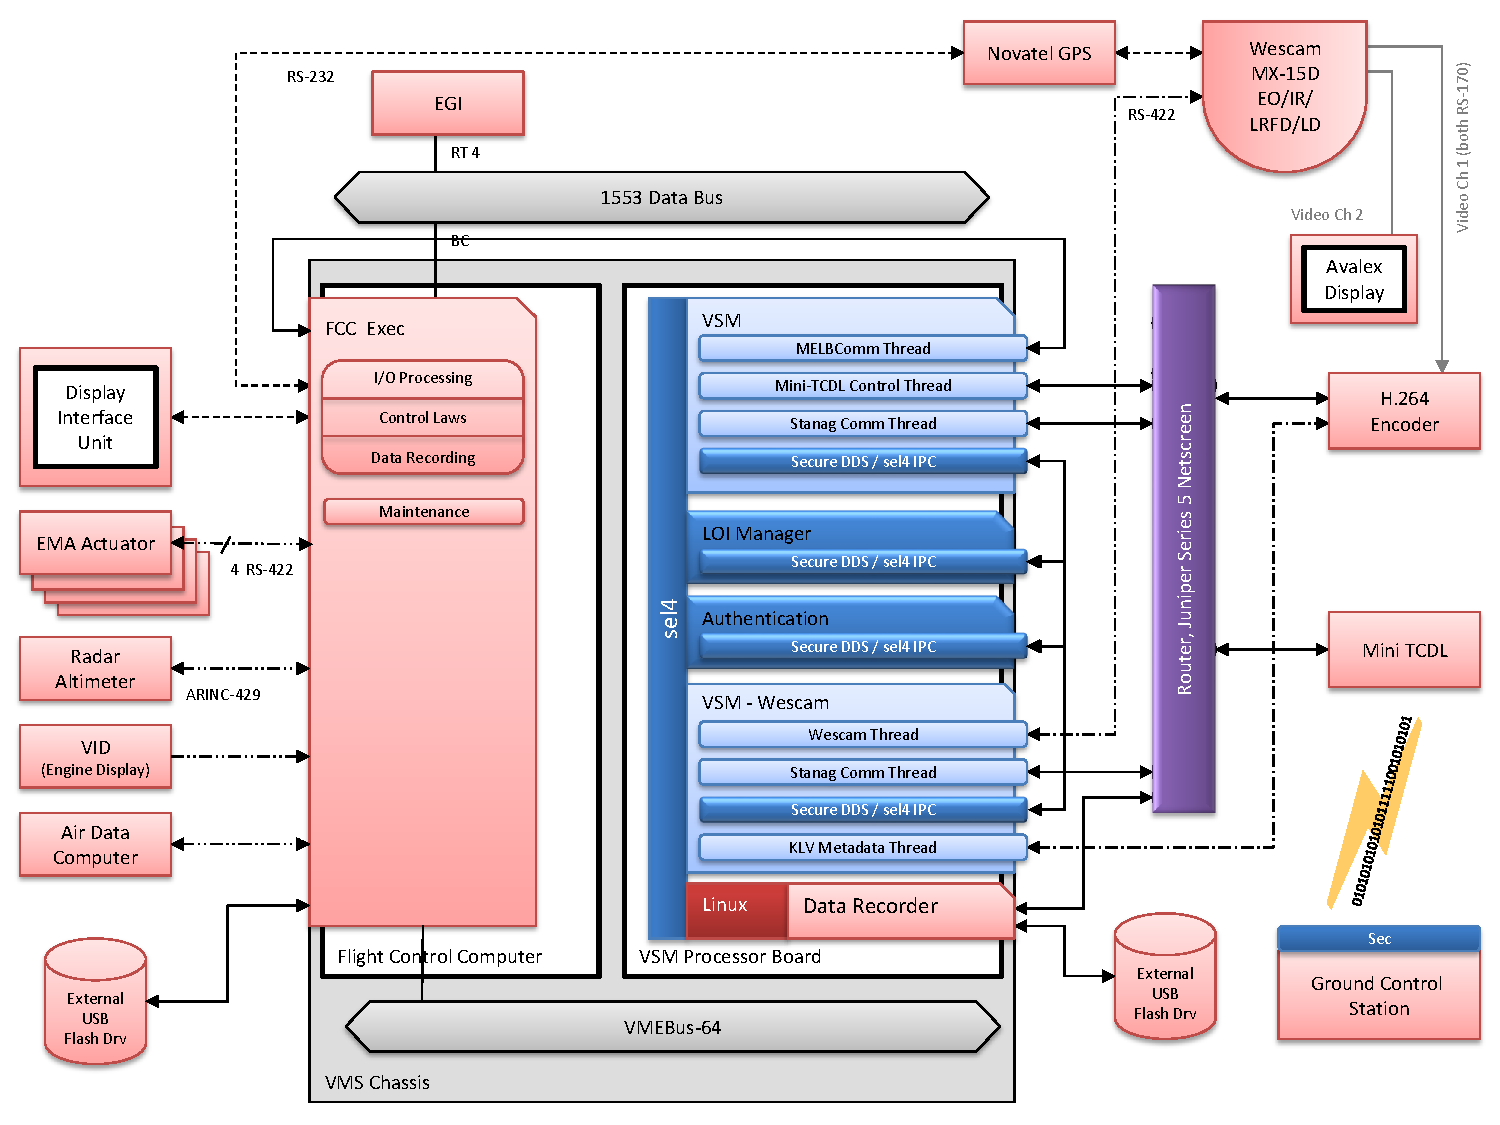
\includegraphics[scale=0.4]{ulb-arch.pdf}
\end{center}
\caption{The Phase II ULB Architecture *Thanks to Boeing for the Figure}
\label{fig:arch}
\end{figure}

Figure~\ref{fig:arch} is not completely isomorphic to the AADL architecture.  Other design decisions have been made since the figure was created that affect the communication mechanisms between different software components.  For example, the LOI Manager directly processes STANAG messages and then passes them on to other components.  The Authentication Component is responsible for decrypting/encrypting messages received and sent from the LOI manager.

We had to modify Boeing's AADL architecture slightly in order to reason about it with AGREE. Specifically, we currently do not have mechanisms in AGREE to reason about bidirectional connections.  We replaced bidirectional connections with two corresponding unidirectional connections.  This restriction is something we plan to address in the future.

\section{Overview of AGREE}

\subsection{Compositional Verification}\label{sec:comp-v}
AGREE is a language and a tool for compositional verification of AADL models.  The behavior of a model is described by \textit{contracts} specified on each component.  A contract contains a set of \textit{assumptions} about the component's inputs and a set of \textit{guarantees} about the component's outputs.  The guarantees of a component are true provided the component's assumptions are true.  The goal of the analysis is to prove that a component's contract is entailed by the contracts of its subcomponents.  Formally, let a system $S : (A,G,C)$ consist of a set of assumptions $A$, guarantees $G$, and subcomponents $C$. We use the notation $S_g$ represent the conjunction of all guarantees of $S$ (i.e., $S_g = \bigwedge_{g \in G} g$) and $S_a$ represent the conjunction of all assumptions of $S$ (i.e., $S_a = \bigwedge_{a \in A} a$). Each subcomponent $c \in C$ is itself a system with assumptions, guarantees, and subcomponents. The goal of our analysis is to prove that a system's guarantees hold as long as its assumptions have always held.  This is stated formally in Formula~\ref{fml:obligation}.

\begin{center}
\begin{equation}\label{fml:obligation}
H(S_a) \rightarrow S_g
\end{equation}
\end{center}

Where the predicate $H$ is true if its argument has held \textit{historically} (i.e., the expression has been true at every time step up until and including now). In order to prove Formula~\ref{fml:obligation} we prove that the assumptions of all the subcomponents of system $S$ hold under the assumptions of $S$.

\begin{center}
\begin{equation}\label{fml:strong-assump}
H(S_a) \rightarrow c_a 
\end{equation}
\end{center}

Formula~\ref{fml:strong-assump} should be shown for each subcomponent $c \in C$. This formula is actually stronger than what we need to prove.  It might be the case that the assumptions of certain subcomponents are satisfied by the guarantees of other subcomponents (and possibly the guarantees of the component itself at previous instances in time).  This weaker condition is shown in Formula~\ref{fml:weak-assump}.

\begin{center}
\begin{equation}\label{fml:weak-assump}
 H(S_a) \wedge Pre(H(c_g))\wedge\bigwedge_{d \in C, c \neq d} H(d_g) \rightarrow c_a 
\end{equation}
\end{center}

Formula~\ref{fml:weak-assump} should be shown for each subcomponent $c \in C$.  This formula is also not quite what we want to prove.  It is not sound in certain scenarios where components are connected immediately in a cyclic manner.  One could imagine a scenario where the assumptions of of two components are true precisely because of the guarantees of the other component (i.e., $c_g \rightarrow d_a $ and $d_g \rightarrow c_a$ for $c,d \in C$ and $c \neq d$). Perhaps components $c$ and $d$ assume that their inputs are positive, and they guarantee that their outputs are positive.  If their outputs are wired to the other's inputs, the state of the system is poorly defined.  To avoid this problem, AGREE actually creates a total ordering of a system's subcomponents.  It uses this ordering to determine which subcomponent guarantees are used to prove the assumptions of other subcomponents.  This slight modification of Formula~\ref{fml:weak-assump} is shown in Formula~\ref{fml:correct-assump}.

\begin{center}
\begin{equation}\label{fml:correct-assump}
 H(S_a) \wedge Pre(H(c_g))\wedge\bigwedge_{d \in C, d < c} H(d_g) \rightarrow c_a 
\end{equation}
\end{center}

In practice this order is determined by the order in which the subcomponents are listed in an AADL component implementation.  Subcomponents listed later are higher in the order than those listed sooner. If Formula~\ref{fml:correct-assump} holds for all subcomponent assumptions then we demonstrate that Formula~\ref{fml:obligation} is true by showing that the system assumptions and subcomponent guarantees satisfy the system guarantees.  Formally, if Formula~\ref{fml:correct-assump} holds for all $c \in C$, then Formula~\ref{fml:guar-check} implies Formula~\ref{fml:obligation}. 

\begin{center}
\begin{equation}\label{fml:guar-check}
 H(S_a) \wedge \bigwedge_{c \in C} H(c_g) \rightarrow S_g 
\end{equation}
\end{center}

\begin{figure}
\begin{center}
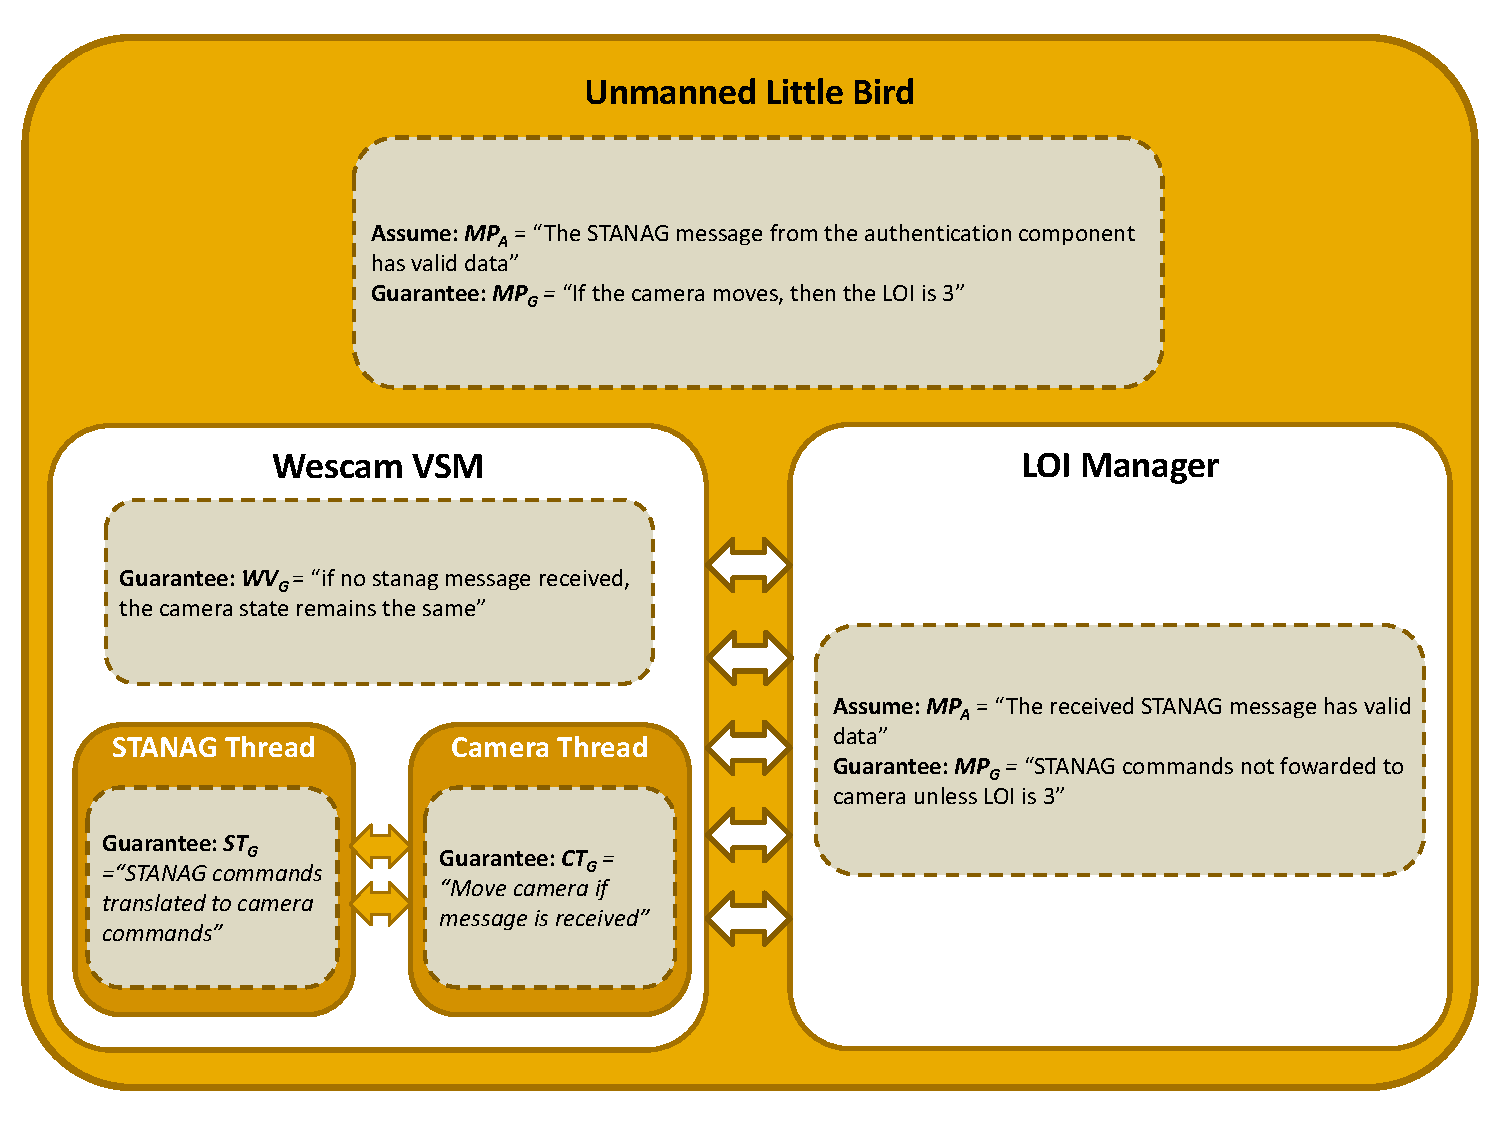
\includegraphics[scale=0.5]{camera_prop.pdf}
\end{center}
\caption{A simplified picture of some of the ULB components with example AGREE contracts}
\label{fig:agree-arch}
\end{figure}

The reader can review~\cite{agree} for rigorous arguments about the correctness of the analysis. To motivate how this analysis is applied to a real-world model, we present a simplified example of a portion of the ULB's AADL model in Figure~\ref{fig:agree-arch}.  At the top of the model's component hierarchy is a system component representing the ULB.  The direct subcomponents of the ULB are the Wescam VSM and the LOI Manager.  The Wescam VSM process contains two threads: the STANAG Thread and the Camera Thread. Each component in the model contains an AGREE contract describing the component's behavior.  For example, the contract of the STANAG Thread running in the Wescam VSM guarantees that information contained in a STANAG message is translated into information that the Camera Thread can understand.  This guarantee is essentially a set of constraints describing how fields of the STANAG message are mapped to fields of an internal message describing the state of the camera.

The guarantees of the STANAG and Camera threads should be sufficient to prove the guarantees of the Wescam VSM.  Specifically, it should be deduced from the contracts of the two threads that ``If no STANAG message is received, then the camera state remains the same''.  In the next section we describe in more detail what we modelled and what we proved about the LOI authorization portion of STANAG 4586 running on the ULB.

\subsection{Modeling Component Execution}

By default, AGREE reasons about a model synchronously. That is, the state of a component is free to change at any instant in time.  However, this constraint might be too strict to be realistic for some systems.  For example, it is not accurate to model multiple threads scheduled to run on the same processor this way.

AGREE can also be used to model quasi-synchronous systems.  A quasi-synchronous system is one in which components run on individual clocks and the relative rates of the clocks are bounded.  For example, one might choose to model two processors that run at the same rate, but have some bounded amount of drift or jitter.  We refer to the constraint on when components' clocks can tick as the ``calendar''. Each component has a calender that determines the order in which its subcomponents execute. We say that a components ``clock ticks'' to refer to the moment in time when its state is allowed to change.

Proving properties compositionally about models with components running on different clock domains is more complex than the methods presented in the previous section.  Informally, the analysis is different in several ways.

\begin{enumerate}
\item The guarantees of a component only hold \textit{once its clock has ticked}.  A component's guarantees are always relative to its own clock. For example, if a component guarantees that ``Its output is one greater than its previous input'', it really means ``when the components clock ticks, its output is one greater than its input immediately before its clock ticked''.

\item Likewise, we only attempt to prove that a component's assumptions hold when the component's clock ticks.

\item In order for the compositional proof to be sound, a component's calendar cannot be \textit{more restrictive} than the calendars of its subcomponents.  In other words, the calendar we choose for a component should abstract the possible orders of executions of all the components lower than it in the hierarchy. This a subtle point, and we do not choose to go into too much detail about it in this document.  Right now AGREE allows the user to manually choose what calendar to use at each component in the hierarchy.  Realistically, the order in which the leaf level components are allowed to execute should determine the calendars of components higher up the model.  Eventually we will change the tool do this automatically.
\end{enumerate}

In the next section we discuss AGREE's syntax.  We explain how the ``synchrony statement'' is used to enforce the relative rates of a components subcomponents.

\subsection{The AGREE Language}

AADL describes the interface of a component in a \textit{component type}. A component type contains a list of \textit{features}, which are the inputs and outputs of a component, and possibly a list of AADL properties.  A \textit{component implementation} is used to describe a specific instance of a component type.  A component implementation contains a list of subcomponents and list of connections that occur between its subcomponents and features.  

For example, one may decide to create a component type for a car which contains features describing its throttle, speed, and direction.  A car component may have many implementations (like a 2006 Toyota Camry, or a McLaren 650s). Different implementations may contain different electronic components, actuators, etc.

AADL contains special syntax elements called \textit{annexes} that can be used to extend the language. The syntax for a component's contract exists in an AGREE annex placed inside of the component type.  AGREE syntax can also be placed inside of annexes in a component implementation or an AADL Package. Syntax placed in an annex in an AADL Package can be used to create libraries that can be referenced by other components.  

Figure~\ref{fig:grammar} shows the simplified description of AGREE's grammar in EBNF. An AGREE annex in an AADL component type contains syntax that is recognized as a \texttt{<contr>} element. Similarly, an AGREE annex in an AADL component implementation contains syntax that is recognized as a \texttt{<impl>} element. The types of statements found in an AADL component type are described below.

\begin{figure}
\begin{grammar}
<contr> ::= <contr-stmt> <contr> | <contr-stmt>

<contr-stmt> ::= `guarantee' <STR> `:' <expr> `;'
\alt `assume' <STR> `:' <expr> `;'
\alt `initially' `:' <expr> `;'
\alt <eq-stmt>
\alt <node-stmt>

<impl> ::= <impl-stmt> <impl> | <impl-stmt>

<impl-stmt> ::= `assert' <expr> `;'
\alt `synchrony' `:' <INT-LIT> (`no_simult')? `;'
\alt `lemma' <STR> `:' <expr> `;'
\alt <eq-stmt>
\alt <node-stmt>

<eq-stmt> ::= `eq' <arg-lst> `=' <expr> `;'
\alt `eq' <arg-lst> `;'

<node-stmnt> ::= `node' <ID> `(' <arg-lst> `)' \\
`returns' `(' <arg-lst> `)' `;' \\
(`var' <arg-lst>)? \\
`let' <eq-lst> `tel' `;'

<expr> ::= <BOOL-LIT>
\alt <INT-LIT>
\alt <REAL-LIT>
\alt <ID>
\alt <ID> `(' <expr-lst> `)'
\alt `pre' `(' <expr> `)'
\alt `event' `(' <ID> `)'
\alt `floor' `(' <expr> `)'
\alt `real' `(' <expr> `)'
\alt `Get_Property' `(' <expr> `,' <aadl-property> `)'
\alt `-' <expr>
\alt `not' <expr>
\alt <expr> `{' <ID> `:=' <expr> `}'
\alt <expr> (`*'|`/'|`mod'|`+'|`-') <expr>
\alt <expr> (`<'|`<='|`>'|`>='|`='|`!=') <expr>
\alt <expr> (`and'|`or') <expr>
\alt <expr> `=>' <expr>
\alt <expr> `->' <expr>

<type> ::= `int' | `real' | `bool' | <aadl-type>

<arg-lst> ::= <ID> `:' <type> `,' <arg-lst> | <ID> `:' <type>

<eq-lst> ::= <eq-stmt> <eq-lst> | <eq-stmt>

<expr-lst> ::= <expr> `,' <expr-lst> | <expr>

\end{grammar}
\caption{A simplified description of the grammar for AGREE}
\label{fig:grammar}
\end{figure}


\begin{itemize}
\item \textbf{Guarantee Statement}: Guarantee statements are proven by the guarantees present in subcomponent contracts.  They in turn are used to prove the guarantees of a components one step above them in the model hierarchy.  These are the guarantees described in Section~\ref{sec:comp-v}.

\item \textbf{Assume Statement}: Assume statements are used to prove the guarantees of the contract as well as the assumptions of the subcomponent contracts. These are the assumptions described in Section~\ref{sec:comp-v}. 

\item \textbf{Initially Statement}: Initially statements are used to constrain the values of the component outputs and intermediate variables before the components clock ever ticks.  This is very subtle and only matters in models that are not synchronous. These statements will make more sense when we explain how we modelled the ULB requirements in Section~\ref{sec:ulb-agree}.

\item \textbf{Equation Statement}: Equation statements are used to define variables.  Variables defined with equation statements are thought of as ``intermediate'' variables or variables that are not meant to be visible in the architectural model (unlike component outputs or inputs).  Equation statements can define variables explicitly by setting the equation equal to an expression immediately after it is defined.  Equation statements can also define variables implicitly by not setting them equal to anything, but constraining them with assumption, assertion, initially, or guarantee statements. Equation statements can actually define more than one variable at once by writing them in a comma delimited list.  One might do this to constrain a list of variables to the results of a node statement that has multiple return values or to more cleanly list a set of implicitly defined variables.

\item \textbf{Node Statement}: Node statements are used to define ``functions'' that might be used frequently in a component type or implementation.  Nodes cannot be recursive or mutually recursive.  Nodes can have multiple return values. If this is the cause, they must be referenced by an equation statement that has multiple arguments. Nodes can also be defined in an AADL Package. If so, they can be referenced in any expression anywhere in the model.  This way one can make a library of certain types of nodes that are useful for different tasks.
\end{itemize}

The \texttt{<expr>} elements in the grammar are very similar to Lustre expressions~\cite{lustre}.  Expressions reason about the current state or past states of variables and can reference variables defined in equation statements or other identifiers in the AADL model. The following is a list of different types of expressions. We describe them in the order they are listed as alternatives to the grammar rule for \texttt{<expr>} in Figure~\ref{fig:grammar}.

\begin{itemize}
\item \textbf{Boolean Literal}: \texttt{true} or \texttt{false}

\item \textbf{Integer Literal}: \texttt{1}, \texttt{42}, \texttt{-1337}, etc \ldots

\item \textbf{Real Literal}: \texttt{3.1415}, \texttt{1.6180}, \texttt{0.001}, etc \ldots

\item \textbf{ID Expression}: An ID is an alpha numeric string (not starting with a number).  ID expressions can also have dots in them (e.g., \texttt{foo.bar.biz}).  ID expressions correspond to variables defined in equation statements or AADL features.  AGREE reasons about the AADL \texttt{Base\_Types::Integer}, \\\texttt{Base\_Types::Float}, and \texttt{Base\_Types::Boolean} as \texttt{int}, \texttt{real}, and \texttt{bool} types, respectively.  ID expressions with dots in them correspond to record types or variables of a subcomponent.  For example, one could use the ID expression \texttt{foo.bar} to reference the input, output, or equation variable \texttt{bar} of subcomponent \texttt{foo} within the implementation of some AADL component. AGREE reasons about AADL Data Implementations like record types.  This will be more clear when we discuss how we modeled the STANAG 4586 messages in Section~\ref{sec:ulb-agree}.

\item \textbf{Node Call Expression}: A node call expression is an ID of a defined node followed by parenthesis.  If the node is defined in an AADL Package, then the ID should be the AADL Package name a dot (\texttt{.}) and then the node name.

\item \textbf{Previous Value Expression}: A previous value expression evaluates to the value of its argument on the previous time frame.  It should that it be guarded by an arrow expressions as its value is undefined on the initial step.

\item \textbf{Event Expression}: An event expression is a special predicate that is used to reason about AADL event data ports.  For an input event data port, its semantics are such that it evaluates to true if a value is \textit{present} on the event port and false otherwise. For an output event data port, its semantics are such that it evaluates true if data is being sent on the port and false otherwise.

\item \textbf{Floor Expression}: A floor expression takes an expression of type \texttt{real} as an argument and returns an \texttt{int} equal to the floor of the number.

\item \textbf{Real Expression}: A real expression takes an expression of type \texttt{int} as argument and returns a \texttt{real} equal to its value.

\item \textbf{Get Property Expression}: A get property expression allows a user to reason about values of AADL properties in the model.  The first argument is the relative path to an AADL component in the instance model or `\texttt{this}' if the property exists in the component in which get property statement lives.  The second argument is the name of the AADL property.

\item \textbf{Minus Expression}: This expression is used to negate integer or real valued expressions.

\item \textbf{Not Expression}: This expression is used to negate boolean valued expressions

\item \textbf{Record Update Expression}: The record update expression expects an expression of record type on the left hand side of the curly braces.  It returns the same record as the left hand side expression except with its member ``ID'' set to the value of the expression on the right hand side of the `\texttt{:=}';

\item \textbf{Arithmetic Operations}: Arithmetic operations must be performed on expressions of the same type.  They follow the standard order of precedence.  Note that AGREE will give a warning if you write an expression that is not linear.  Some theorem provers do not reason about non-linear expressions.  Non-linear integer arithmetic is undecidable and most theorem provers do not use a decidable decision procedure for non-linear real arithmetic.  So it is recommended that you only use linear expressions.

\item \textbf{Relation Expressions}: Relation expressions can be performed on integers or reals, but not a combination of both.  Equality can be used on Booleans as well.

\item \textbf{Boolean Expressions}: Boolean expressions have the standard associative properties and order of precedence. 

\item \textbf{Arrow Expression}: The arrow expression evaluates to the value of the expression of the left hand side of the arrow on the initial step. Otherwise it evaluates to the value of the expression on the right hand side of the arrow.  The arrow expression is used with the \texttt{pre} expression to reason about past values of variables. For example, we can define a variable in an AGREE contract that starts at zero and increments by one each step in time using an equation statement:

\begin{center}
{\color{color18} \textbf{eq}} count {\color{color18} \textbf{:}} {\color{color18} \textbf{int = }} 0 {\color{color18} \textbf{-\texttt{>}}}
{\color{color18} \textbf{pre(}} count {\color{color18} \textbf{)}} + 1
\end{center}

Note that the difference between arrow expressions and the initially statements discussed earlier is very subtle.  Before a subcomponents clock ticks the values of its outputs and intermediate variables defined by equation statements are only constrained by the expressions in initially statements.  Once the subcomponents clock ticks for the first time the expressions in the initially statements become irrelevant and all arrow expressions in the subcomponent evaluate to the value of their left hand side expression.

\end{itemize}  


While assumption and guarantee statements exclusively live in component types, component implementations exclusively contain other grammar elements. Specifically, component implementations can contain the following elements.

\begin{itemize}
\item \textbf{Synchrony Statement}: Synchrony statements describe the order in which the subcomponents execute.  Right now we support modeling systems synchronously or quasi-synchronously.  The synchrony statement expects an integer value which indicates the number of times a subcomponent's clock can tick since any other clock has ticked.  The phrase \texttt{no\_simult} can optionally be placed at the end of the statement to indicate that no two subcomponent clocks may tick simultaneously.  This would be indicative of multiple threads scheduled to run on a single processor for example.

\item \textbf{Assert Statement}: Assert statements make unchecked statements about how the component behaves.  These are also used to reference variables from a subcomponent in the component contract.  For the purpose of analysis assertions are treated just like the system assumptions in the formulas presented in Section~\ref{sec:comp-v}.  However, we never verify that the assertions actually hold.  That is to say, the assertions of a subcomponent are never proven to hold like subcomponent assumptions in Formula~\ref{fml:correct-assump}.  Assertions can be thought of as unchecked assumptions about the behavior of component. Assert statements can refer to equations or features defined in the component type. They are often used to refer to subcomponent variables in contracts higher up in the model hierarchy. We show examples of this in Section~\ref{sec:ulb-agree}.

\item \textbf{Lemma Statement}: Lemma statements are proven just like guarantees.  These are used to help the model checker learn facts to improve its ability to prove other properties.  They differ from guarantees in that subcomponent lemmas are not used to prove other subcomponent guarantees or system guarantees.  In other words, lemmas only ever appear as system guarantees on the right hand side of the implication in Formula~\ref{fml:guar-check}.
\end{itemize}

\section{Modeling the ULB with AGREE}~\label{sec:ulb-agree}

\subsection{The ULB System Component}


\begin{figure}

\noindent\fbox{%
    \parbox{\textwidth}{%
{\color{color17} -{}-points to the decrypted stanag messages}

{\color{color18} \textbf{eq}} auth\_in {\color{color18} \textbf{:}} ULB\_Device\_Types{\color{color18} \textbf{::}}STANAG\_4586\_message{\color{color18} \textbf{.}}cucs\_auth\_req{\color{color18} \textbf{;}}

{\color{color18} \textbf{eq}} stanag\_in {\color{color18} \textbf{:}} ULB\_Device\_Types{\color{color18} \textbf{::}}STANAG\_4586\_message{\color{color18} \textbf{.}}i{\color{color18} \textbf{;}}

\vspace{12pt}
{\color{color18} \textbf{eq}} loi {\color{color18} \textbf{:}} {\color{color18} \textbf{int;}}

{\color{color18} \textbf{eq}} override\_control {\color{color18} \textbf{:}} {\color{color18} \textbf{bool;}}

{\color{color18} \textbf{eq}} cucs\_id {\color{color18} \textbf{:}} {\color{color18} \textbf{int;}}

{\color{color18} \textbf{eq}} camera\_commands {\color{color18} \textbf{:}} ULB\_Device\_Types{\color{color18} \textbf{::}}camera\_command{\color{color18} \textbf{.}}i{\color{color18} \textbf{;}}

{\color{color18} \textbf{eq}} stanag\_received {\color{color18} \textbf{:}} {\color{color18} \textbf{bool;}} 

\vspace{12pt}
{\color{color18} \textbf{guarantee}} {\color{color19} \texttt{"}allowed to override\texttt{"}} 
{\color{color18} \textbf{:}} {\color{color18} \textbf{true}} {\color{color18} \textbf{-\texttt{>} 
 }}

\parindent=7pt
stanag\_received {\color{color18} \textbf{and}}    

stanag\_in{\color{color18} \textbf{.}}m\_id {\color{color18} \textbf{=}} 1 {\color{color18} \textbf{and}} 
  

\parindent=0pt
{\color{color18} \textbf{not}} {\color{color18} \textbf{pre(}}override\_control{\color{color18} \textbf{)}} 
{\color{color18} \textbf{and}}   

\parindent=7pt
auth\_in{\color{color18} \textbf{.}}csm {\color{color18} \textbf{=}} 2     

\parindent=0pt
{\color{color18} \textbf{=\texttt{>}}} cucs\_id {\color{color18} \textbf{=}} auth\_in{\color{color18} \textbf{.}}cucsid{\color{color18} \textbf{; 
 }}

\vspace{12pt}
{\color{color18} \textbf{eq}} message\_with\_loi\_gt\_3 {\color{color18} \textbf{:}} 
{\color{color18} \textbf{bool}} {\color{color18} \textbf{=}}    

\parindent=10pt
stanag\_received {\color{color18} \textbf{and}} stanag\_in{\color{color18} \textbf{.}}m\_id 
{\color{color18} \textbf{=}} 1 {\color{color18} \textbf{and}}    

\parindent=0pt
{\color{color18} \textbf{(}}auth\_in{\color{color18} \textbf{.}}csm {\color{color18} \textbf{=}} 
1 {\color{color18} \textbf{or}} auth\_in{\color{color18} \textbf{.}}csm {\color{color18} \textbf{=}} 
2{\color{color18} \textbf{)}}   {\color{color18} \textbf{and}} auth\_in{\color{color18} \textbf{.}}rloi 
{\color{color18} \textbf{\texttt{>}}} 3{\color{color18} \textbf{;      }}

\vspace{12pt}
{\color{color18} \textbf{guarantee}} {\color{color19} \texttt{"}loi greater than 
three always gets control\texttt{"}} {\color{color18} \textbf{:  }}

\parindent=7pt
message\_with\_loi\_gt\_3 {\color{color18} \textbf{and}} {\color{color18} \textbf{(false}} 
{\color{color18} \textbf{-\texttt{>}}} {\color{color18} \textbf{pre(}}loi {\color{color18} \textbf{=}} 
3{\color{color18} \textbf{))}} {\color{color18} \textbf{=\texttt{>}    }}

\parindent=14pt
loi {\color{color18} \textbf{=}} auth\_in{\color{color18} \textbf{.}}rloi {\color{color18} \textbf{and}} 
cucs\_id {\color{color18} \textbf{=}} auth\_in{\color{color18} \textbf{.}}cucsid{\color{color18} \textbf{;}}

\vspace{12pt}
\parindent=0pt
{\color{color18} \textbf{eq}} loi\_was\_3 {\color{color18} \textbf{:}} {\color{color18} \textbf{bool}} 
{\color{color18} \textbf{=}} loi {\color{color18} \textbf{=}} 3 {\color{color18} \textbf{-\texttt{>}}} 
loi {\color{color18} \textbf{=}} 3 {\color{color18} \textbf{or}} {\color{color18} \textbf{pre(}}loi\_was\_3{\color{color18} \textbf{);}}

\vspace{12pt}
{\color{color18} \textbf{guarantee}} {\color{color19} \texttt{"}if the camera moved, 
then loi was three\texttt{"}}{\color{color18} \textbf{:}} {\color{color18} \textbf{true}} 
{\color{color18} \textbf{-\texttt{>}  }}

\parindent=7pt
camera\_commands {\color{color18} \textbf{!=}} {\color{color18} \textbf{pre(}}camera\_commands{\color{color18} \textbf{)}} 
{\color{color18} \textbf{=\texttt{>}}} loi\_was\_3{\color{color18} \textbf{;}}
{\color{color18} \textbf{;}}

}%
}
\caption{The contract in the ULB}
\label{fig:ulb}
\end{figure}

As mentioned earlier, the FCC VSM, LOI Manager, Authentication Component, and Wescam VSM are modelled as process components in AADL. A process in AADL is thought of as an isolated memory space whereas a thread is used to describe computation that takes place within a process.  We model the LOI Manager and Authentication Component as processes without any threads, but it is assumed that each process has some sort of ``main thread'' which performs its execution.  We could model this explicitly; each process would have a single thread with the same assumptions and guarantees as the process itself.  We have omitted this detail in the model.

Figure~\ref{fig:ulb} shows the highest level contract of the model (contained in the ULB system component).  The contract has three guarantees which are proven by the contracts of the LOI Manager, the Wescam VSM, and the Authentication Component.  These guarantees are meant to capture the following English requirements:
\begin{enumerate}
\item If a STANAG 4586 message is received, and the CUCS is asserting to override control, and the previous CUCS did not assert control, then the new CUCS is granted control.

\item If the current CUCS in control has LOI of 3, a CUCS requesting control with a higher LOI is granted access.

\item If the camera changes state, then the LOI was 3.
\end{enumerate}

\begin{figure}

\noindent\fbox{%
    \parbox{\textwidth}{%

{\color{color18} \textbf{synchrony:}} 5 {\color{color18} \textbf{no\_simult;}}

\vspace{12pt}
{\color{color18} \textbf{eq}} loi\_clk {\color{color18} \textbf{:}} {\color{color18} \textbf{bool;}}

{\color{color18} \textbf{eq}} cam\_clk {\color{color18} \textbf{:}} {\color{color18} \textbf{bool;}}

{\color{color18} \textbf{assert}} loi\_clk {\color{color18} \textbf{=}} loi\_sw{\color{color18} \textbf{.\_CLK;}}

{\color{color18} \textbf{assert}} cam\_clk {\color{color18} \textbf{=}} wescam\_vsm\_sw{\color{color18} \textbf{.\_CLK;}}

\vspace{12pt}
{\color{color17} -{}-grabbing variables out of subcomponents}

{\color{color18} \textbf{assert}} loi\_sw{\color{color18} \textbf{.}}id\_in\_control 
{\color{color18} \textbf{=}} cucs\_id{\color{color18} \textbf{;}}

{\color{color18} \textbf{assert}} loi\_sw{\color{color18} \textbf{.}}override\_control 
{\color{color18} \textbf{=}} override\_control{\color{color18} \textbf{;}}

{\color{color18} \textbf{assert}} loi\_sw{\color{color18} \textbf{.}}loi {\color{color18} \textbf{=}} 
loi{\color{color18} \textbf{;}}

{\color{color18} \textbf{assert}} loi\_sw{\color{color18} \textbf{.}}outside\_stanag\_in 
{\color{color18} \textbf{=}} stanag\_in{\color{color18} \textbf{;}}

{\color{color18} \textbf{assert}} loi\_sw{\color{color18} \textbf{.}}outside\_stanag\_in{\color{color18} \textbf{.}}m\_data{\color{color18} \textbf{.}}cucs\_auth\_req 
{\color{color18} \textbf{=}} auth\_in{\color{color18} \textbf{;}}

{\color{color18} \textbf{assert}} wescam\_vsm\_sw{\color{color18} \textbf{.}}camera\_commands 
{\color{color18} \textbf{=}} camera\_commands{\color{color18} \textbf{;}}

{\color{color18} \textbf{assert}} stanag\_received {\color{color18} \textbf{=}} 
{\color{color18} \textbf{(event(}}loi\_sw{\color{color18} \textbf{.}}outside\_stanag\_in{\color{color18} \textbf{)}} 
{\color{color18} \textbf{and}} loi\_clk{\color{color18} \textbf{);}}       

\vspace{12pt}
{\color{color17} -{}-wescam vsm sees all messages sent to it}

{\color{color18} \textbf{assert}} {\color{color18} \textbf{(true}} {\color{color18} \textbf{-\texttt{>}}} 
{\color{color18} \textbf{(pre(event(}}wescam\_vsm\_sw{\color{color18} \textbf{.}}stanag\_in{\color{color18} \textbf{))}} 
{\color{color18} \textbf{and}} {\color{color18} \textbf{not}} {\color{color18} \textbf{pre(}}cam\_clk{\color{color18} \textbf{)) 
 }}
{\color{color18} \textbf{=\texttt{>}}} {\color{color18} \textbf{(}}wescam\_vsm\_sw{\color{color18} \textbf{.}}stanag\_in 
{\color{color18} \textbf{=}} {\color{color18} \textbf{pre(}}wescam\_vsm\_sw{\color{color18} \textbf{.}}stanag\_in{\color{color18} \textbf{)}} 
{\color{color18} \textbf{and}}      

{\color{color18} \textbf{event(}}wescam\_vsm\_sw{\color{color18} \textbf{.}}stanag\_in{\color{color18} \textbf{)}} 
{\color{color18} \textbf{=}} {\color{color18} \textbf{true));        }}

\vspace{12pt}
{\color{color18} \textbf{lemma}} {\color{color19} \texttt{"}if the wescam gets 
a message, then the loi is 3\texttt{"}} {\color{color18} \textbf{:  }}

{\color{color18} \textbf{event(}}wescam\_vsm\_sw{\color{color18} \textbf{.}}stanag\_in{\color{color18} \textbf{)}} 
{\color{color18} \textbf{=\texttt{>}}} loi {\color{color18} \textbf{=}} 3{\color{color18} \textbf{;}}

\vspace{12pt}
{\color{color18} \textbf{lemma}} {\color{color19} \texttt{"}if the loi was never 
3, then an event was never sent to the wescam\texttt{"}} {\color{color18} \textbf{: 
 }}

\baselineskip=13pt
{\color{color18} \textbf{not}} loi\_was\_3 {\color{color18} \textbf{=\texttt{>}}} 
{\color{color18} \textbf{not}} wescam\_vsm\_sw{\color{color18} \textbf{.}}event\_in\_past{\color{color18} \textbf{;}}

}%
}
\caption{Assert statements in the ULB implementation}
\label{fig:ulb-impl}
\end{figure}

Figure~\ref{fig:ulb-impl} shows the assertions, synchrony statement, and lemmas defined in the ULB implementation. We use assert statements in the ULB implementation to refer to variables present in the ULB's subcomponents.  Because AGREE only performs analysis at one level of the hierarchy at a time, this technique can be used to manually refer to information about leaf level components at higher tiers in the hierarchy.  Specifically, we assert that the \texttt{stanag\_received} variable defined in the contract is true if and only if the LOI Manager is currently executing and it received a STANAG message.  We also assert the equivalence of the \texttt{loi}, \texttt{cucs\_id}, \texttt{override\_control}, \texttt{stanag\_in}, etc\ldots variables in the LOI Manager with their corresponding variables in the ULB contract.

We assert that every STANAG message sent to the Wescam VSM is handled by the Wescam VSM before another message is sent to it.  This may not be true of the actual implementation.  We could possibly model some sort of queue to handle multiple messages being received by the Wescam VSM, but it would make proving properties more complicated.

The synchrony statement listed in the ULB implementation describes the order in which the subcomponents of the ULB execute. The integer argument in the statement indicates how many time a component's clock can tick in reference to the clock of every other component.  In this case we somewhat arbitrarily chose 5.  For example, the LOI Manager process can execute no more than 5 times since the Wescam VSM and Authentication Component have last executed.  The phrase ``no\_simult'' at the end of the synchrony statements indicates that no two clocks may tick simultaneously.  This reflects the fact that all of the processes that we have modelled so far run on the same processor.  The clock variables of individual components can be referred to by referencing the reserved variable ``\_CLK'' in the subcomponent.  For example, we have an assert statement saying that the variable \texttt{loi\_clk} is equivalent to the clock variable of the LOI Manager.

Lemma statements are used to help the model checker prove the ULB's guarantees.  Specifically, the lemma stating ``If the LOI was never 3, then an event was never sent to the wescam'' is used as a suggested invariant to help prove the guarantee ``If the camera moved, then the LOI was three''.  Depending on the power of the model checker these lemmas may not be necessary to prove the guarantees, but they always have the added utility of proving more facts about the ULB.

\subsection{The Authentication Component}

The contract for the Authentication Component is shown in Figure~\ref{fig:auth-contract}.  The component guarantees that any authorization message that it passes on to the LOI Manager has valid data. By valid data we mean that specific fields in an authorization message are within the ranges specified by the STANAG 4586 specification. This is needed to prove the assumption listed in the LOI Manager\footnote{We list the LOI Manager last in the order of subcomponents in the ULB implementation so that it is higher in the total ordering for proving assumptions}.

We represented different STANAG 4586 message types by including multiple subcomponents within the STANAG 4586 message data implementation. This is shown in Figure~\ref{fig:stanag-data}.  Implementing the message data this way is similar to how someone would implement it as a structure in the C language using a union for different structures over the message data field.  In the contract for the Authorization Component we use the variable \texttt{auth\_in} to specifically reference this portion of the STANAG 4586 message data field.

We use an initially statement to say that before the component's clock ticks it has no events being sent on its STANAG output.

\begin{figure}
\noindent\fbox{%
    \parbox{\textwidth}{%
{\color{color18} \textbf{eq}} auth\_in {\color{color18} \textbf{:}} ULB\_Device\_Types{\color{color18} \textbf{::}}STANAG\_4586\_message{\color{color18} \textbf{.}}cucs\_auth\_req 
 

\parindent=10pt
{\color{color18} \textbf{=}} stanag\_onboard\_out{\color{color18} \textbf{.}}m\_data{\color{color18} \textbf{.}}cucs\_auth\_req{\color{color18} \textbf{; 
 }}

\parindent=0pt
\vspace{12pt}
{\color{color18} \textbf{initially:   }}

\parindent=10pt
{\color{color18} \textbf{not}} {\color{color18} \textbf{event(}}stanag\_onboard\_out{\color{color18} \textbf{); 
    }}

\vspace{12pt}
\parindent=0pt
{\color{color18} \textbf{guarantee}} {\color{color19} \texttt{"}valid auth data\texttt{"}} 
{\color{color18} \textbf{:   }}

\parindent=10pt
0 {\color{color18} \textbf{\texttt{<}}} auth\_in{\color{color18} \textbf{.}}rloi 
{\color{color18} \textbf{and}} auth\_in{\color{color18} \textbf{.}}rloi {\color{color18} \textbf{\texttt{<}=}} 
5 {\color{color18} \textbf{and   }}

0 {\color{color18} \textbf{\texttt{<}=}} auth\_in{\color{color18} \textbf{.}}csm 
{\color{color18} \textbf{and}} auth\_in{\color{color18} \textbf{.}}csm {\color{color18} \textbf{\texttt{<}=}} 
2 {\color{color18} \textbf{and   }}

0 {\color{color18} \textbf{\texttt{<}}} auth\_in{\color{color18} \textbf{.}}cucsid 
{\color{color18} \textbf{and}} auth\_in{\color{color18} \textbf{.}}cucsid {\color{color18} \textbf{\texttt{<}}} 
255 {\color{color18} \textbf{and   }}

\parindent=0pt
{\color{color17} -{}-right now we model just two control stations    }

\baselineskip=13pt
\parindent=10pt
0 {\color{color18} \textbf{\texttt{<}=}} auth\_in{\color{color18} \textbf{.}}cs 
{\color{color18} \textbf{and}} auth\_in{\color{color18} \textbf{.}}cs {\color{color18} \textbf{\texttt{<}=}} 
1{\color{color18} \textbf{;}}

}%
}
\caption{The contract for the Authentication Component}
\label{fig:auth-contract}
\end{figure}

\begin{figure}
\noindent\fbox{%
    \parbox{\textwidth}{%

{\color{color18} \textbf{data}} STANAG\_4586\_message  

{\color{color18} \textbf{end}} STANAG\_4586\_message;    

\vspace{12pt}
{\color{color18} \textbf{data}} {\color{color18} \textbf{implementation}} STANAG\_4586\_message.i 
   

{\color{color18} \textbf{subcomponents      }}

\parindent=21pt
m\_id : {\color{color18} \textbf{data}} Base\_Types::Integer;      

m\_data : {\color{color18} \textbf{data}} STANAG\_4586\_message\_data.i;  

\parindent=0pt
{\color{color18} \textbf{end}} STANAG\_4586\_message.i;    

\vspace{12pt}
{\color{color18} \textbf{data}} STANAG\_4586\_message\_data  

{\color{color18} \textbf{end}} STANAG\_4586\_message\_data;    

\vspace{12pt}
{\color{color18} \textbf{data}} {\color{color18} \textbf{implementation}} STANAG\_4586\_message\_data.i 
   

{\color{color18} \textbf{subcomponents      }}

\parindent=21pt
cucs\_auth\_req : {\color{color18} \textbf{data}} STANAG\_4586\_message.cucs\_auth\_req; 
     

payload\_steer : {\color{color18} \textbf{data}} STANAG\_4586\_message.payload\_steer; 
 

\parindent=0pt
{\color{color18} \textbf{end}} STANAG\_4586\_message\_data.i;    

\vspace{12pt}
{\color{color18} \textbf{data}} {\color{color18} \textbf{implementation}} STANAG\_4586\_message.cucs\_auth\_req 
   

{\color{color18} \textbf{subcomponents      }}

\parindent=21pt
tstamp : {\color{color18} \textbf{data}} Base\_Types::Integer;      

vid : {\color{color18} \textbf{data}} Base\_Types::Integer;      

cucsid : {\color{color18} \textbf{data}} Base\_Types::Integer;      

vtype : {\color{color18} \textbf{data}} Base\_Types::Integer;      

vsubtype : {\color{color18} \textbf{data}} Base\_Types::Integer;      

dlid : {\color{color18} \textbf{data}} Base\_Types::Integer;      

rloi : {\color{color18} \textbf{data}} Base\_Types::Integer;      

cs : {\color{color18} \textbf{data}} Base\_Types::Integer;      

csm : {\color{color18} \textbf{data}} Base\_Types::Integer;      

wait : {\color{color18} \textbf{data}} Base\_Types::Integer;  

\parindent=0pt
{\color{color18} \textbf{end}} STANAG\_4586\_message.cucs\_auth\_req;

}%
}
\caption{The AADL data implementation for STANAG 4586 message}
\label{fig:stanag-data}
\end{figure}

\subsection{The LOI Manager}

The AGREE annex in the LOI Manager houses the majority of the logic in the model.  The assumptions and guarantees that are present in the process were derived from the STANAG 4586 specification and from discussions with Boeing. In order to fit the annex cleanly into this document we split the contract into five pieces shown in Figures~\ref{fig:loi-contract1},~\ref{fig:loi-contract2},~\ref{fig:loi-contract3},~\ref{fig:loi-contract4}, and~\ref{fig:loi-contract5}. Figure~\ref{fig:loi-contract1} shows the intermediate variables defined in the annex.  The LOI Manager keeps track of the current LOI, the CUCS in control, whether or not the CUCS has asserted that it is overriding control, and which control station the CUCS is controlling.

In Figure~\ref{fig:loi-contract2} we define the variable \texttt{loi\_approved\_for\_message} to be true if the current message type is correct with respect to the LOI that has been authorized. Whether or not a specific message ID is authorized at a particular LOI level comes directly from the STANAG 4586 specification. This variable is used to determine whether or not a message is routed to either of the VSMs or if the message is ignored.  In total, the LOI Manager makes three guarantees.

\begin{enumerate}
\item If no message is received, or the message that is received is not an authorization request, then all of the LOI state variables remain the same.  This property is likely implicit to any software implementation of the component, but we must make explicit or else the model checker will choose non-deterministic values for these variables.

\item If a message is received and it is an authorization request, then it is handled according to the STANAG 4586 specification.  Specifically this guarantee covers the following scenarios:

\begin{enumerate}
\item If the CUCS who is in control is relinquishing control, then no one is overriding control, no one is in control, and the LOI is set to zero\footnote{Setting the LOI to zero is not explicit in the specification, but it needs to be set to some non-permissive value}.

\item If a CUCS is requesting control or attempting to override control and the previous LOI is 3 and the requested LOI is greater than 3, then the CUCS is granted control.

\item If a CUCS is requesting control and no CUCS is currently overriding control, then the CUCS is granted control.

\item If a CUCS is attempting to override control and no CUCS is currently overriding control, then the CUCS overrides control.
\end{enumerate}

\item If the a message is received and the current LOI is approved for the message type, then it is fowarded to the Wescam VSM if the LOI is 3 and the control station is set to the Wescam VSM\footnote{These restrictions about the control station are based on Boeing's requirements and not part of the STANAG 4586 specification. The specification states that camera control commands require LOI of 3}.  Otherwise, the message is forwarded to the FCC VSM.  If no message is received or if the message is not approved at the current LOI then the message is not fowarded to either VSM.

\end{enumerate}

These guarantees could possibly be broken out into smaller requirements rather than large nested ``if then else'' blocks.  This is more of a choice of style / readability. The LOI Manager assumes that the data fields for authorization messages are in their correct ranges.  This assumption should be satisfied by guarantees from the Authentication Component.

The LOI Manager implementation provided by Boeing includes logic for searching through a list of pre-authorized CUCS to determine whether or not the requesting CUCS can obtain a certain LOI.  We did not explicitly model this with our requirements.  Although, it could be trivially added by creating a boolean variable that indicates whether or not the requesting CUCS was present in the list and has permissions for the requested LOI.  One could even model the list in AGREE if desired.  The best solution might be to just include this ``CUCS is allowed requested LOI'' variable in the guarantees and then make it an obligation on the component designer that lookup works correctly.

\begin{figure}

\noindent\fbox{%
    \parbox{\textwidth}{%

{\color{color18} \textbf{eq}} loi {\color{color18} \textbf{:}} {\color{color18} \textbf{int;}}

{\color{color18} \textbf{eq}} auth\_in {\color{color18} \textbf{:}} ULB\_Device\_Types{\color{color18} \textbf{::}}STANAG\_4586\_message{\color{color18} \textbf{.}}cucs\_auth\_req 
  

{\color{color18} \textbf{=}} outside\_stanag\_in{\color{color18} \textbf{.}}m\_data{\color{color18} \textbf{.}}cucs\_auth\_req{\color{color18} \textbf{;}} 

{\color{color18} \textbf{eq}} id\_in\_control {\color{color18} \textbf{:}} {\color{color18} \textbf{int;}} 

{\color{color18} \textbf{eq}} override\_control {\color{color18} \textbf{:}} {\color{color18} \textbf{bool;}}

{\color{color18} \textbf{eq}} none\_in\_control {\color{color18} \textbf{:}} {\color{color18} \textbf{bool;}} 

{\color{color18} \textbf{eq}} control\_station {\color{color18} \textbf{:}} {\color{color18} \textbf{int;}}

{\color{color17} -{}-in the actual implementation this should be ascertained}

{\color{color17} -{}-by checking to see if the CUCS is in the auth\_map with}

{\color{color17} -{}-a specified loi}

{\color{color18} \textbf{eq}} is\_auth\_loi {\color{color18} \textbf{:}} {\color{color18} \textbf{bool;}}

\vspace{12pt}
{\color{color18} \textbf{eq}} mid {\color{color18} \textbf{:}} {\color{color18} \textbf{int}} 
{\color{color18} \textbf{=}} outside\_stanag\_in{\color{color18} \textbf{.}}m\_id{\color{color18} \textbf{;}}

\vspace{12pt}
{\color{color18} \textbf{eq}} loi2 {\color{color18} \textbf{:}} {\color{color18} \textbf{bool}} 
{\color{color18} \textbf{=}} loi {\color{color18} \textbf{=}} 2{\color{color18} \textbf{;}}

{\color{color18} \textbf{eq}} loi3 {\color{color18} \textbf{:}} {\color{color18} \textbf{bool}} 
{\color{color18} \textbf{=}} loi {\color{color18} \textbf{=}} 3{\color{color18} \textbf{;}}

{\color{color18} \textbf{eq}} loi45 {\color{color18} \textbf{:}} {\color{color18} \textbf{bool}} 
{\color{color18} \textbf{=}} loi {\color{color18} \textbf{=}} 4 {\color{color18} \textbf{or}} 
loi {\color{color18} \textbf{=}} 5{\color{color18} \textbf{;  }}

}%
}
\caption{Part 1 of the contract for the LOI Manager}
\label{fig:loi-contract1}
\end{figure}


\begin{figure}
\vspace{-40pt}

\noindent\fbox{%
    \parbox{\textwidth}{%

{\color{color18} \textbf{eq}} loi\_approved\_for\_message {\color{color18} \textbf{:}} 
{\color{color18} \textbf{bool  }}
 {\color{color18} \textbf{=}} 
{\color{color18} \textbf{(  }}

{\color{color18} \textbf{if(}}mid {\color{color18} \textbf{=}} 1{\color{color18} \textbf{)}} 
{\color{color18} \textbf{then}} {\color{color17} -{}-note that this is an auth request, 
so we don't route it    }

{\color{color18} \textbf{false  }}

{\color{color18} \textbf{else}} {\color{color18} \textbf{if(}}mid {\color{color18} \textbf{=}} 
20 {\color{color18} \textbf{or}} mid {\color{color18} \textbf{=}} 21{\color{color18} \textbf{)}} 
{\color{color18} \textbf{then    }}

\parindent=14pt
loi2 {\color{color18} \textbf{or}} loi3 {\color{color18} \textbf{or}} loi45  

\parindent=0pt
{\color{color18} \textbf{else}} {\color{color18} \textbf{if(}}40 {\color{color18} \textbf{\texttt{<}=}} 
mid {\color{color18} \textbf{and}} mid {\color{color18} \textbf{\texttt{<}=}} 46{\color{color18} \textbf{)}} 
{\color{color18} \textbf{then    }}

\parindent=14pt
loi45  

\parindent=0pt
{\color{color18} \textbf{else}} {\color{color18} \textbf{if(}}mid {\color{color18} \textbf{=}} 
47{\color{color18} \textbf{)}} {\color{color18} \textbf{then    }}

\parindent=14pt
loi3 {\color{color18} \textbf{or}} loi45  

\parindent=0pt
{\color{color18} \textbf{else}} {\color{color18} \textbf{if(}}mid {\color{color18} \textbf{=}} 
100{\color{color18} \textbf{)}} {\color{color18} \textbf{then    }}

\parindent=14pt
loi45  

\parindent=0pt
{\color{color18} \textbf{else}} {\color{color18} \textbf{if(}}mid {\color{color18} \textbf{=}} 
101{\color{color18} \textbf{)}} {\color{color18} \textbf{then    }}

\parindent=14pt
loi2 {\color{color18} \textbf{or}} loi3 {\color{color18} \textbf{or}} loi45  

\parindent=0pt
{\color{color18} \textbf{else}} {\color{color18} \textbf{if(}}102 {\color{color18} \textbf{\texttt{<}=}} 
mid {\color{color18} \textbf{and}} mid {\color{color18} \textbf{\texttt{<}=}} 108{\color{color18} \textbf{)}} 
{\color{color18} \textbf{then    }}

\parindent=14pt
loi45  

\parindent=0pt
{\color{color18} \textbf{else}} {\color{color18} \textbf{if(}}200 {\color{color18} \textbf{\texttt{<}=}} 
mid {\color{color18} \textbf{and}} mid {\color{color18} \textbf{\texttt{<}=}} 206{\color{color18} \textbf{)}} 
{\color{color18} \textbf{then    }}

\parindent=14pt
loi3  

\parindent=0pt
{\color{color18} \textbf{else}} {\color{color18} \textbf{if(}}mid {\color{color18} \textbf{=}} 
207{\color{color18} \textbf{)}} {\color{color18} \textbf{then    }}

\parindent=14pt
loi3 {\color{color18} \textbf{or}} loi45  

\parindent=0pt
{\color{color18} \textbf{else}} {\color{color18} \textbf{if(}}300 {\color{color18} \textbf{\texttt{<}=}} 
mid {\color{color18} \textbf{and}} mid {\color{color18} \textbf{\texttt{<}=}} 306{\color{color18} \textbf{)}} 
{\color{color18} \textbf{then    }}

\parindent=14pt
loi2 {\color{color18} \textbf{or}} loi3  

\parindent=0pt
{\color{color18} \textbf{else}} {\color{color18} \textbf{if(}}mid {\color{color18} \textbf{=}} 
307 {\color{color18} \textbf{or}} mid {\color{color18} \textbf{=}} 308{\color{color18} \textbf{)}} 
{\color{color18} \textbf{then    }}

\parindent=14pt
loi3  

\parindent=0pt
{\color{color18} \textbf{else}} {\color{color18} \textbf{if(}}400 {\color{color18} \textbf{\texttt{<}=}} 
mid {\color{color18} \textbf{and}} mid {\color{color18} \textbf{\texttt{<}=}} 404{\color{color18} \textbf{)}} 
{\color{color18} \textbf{then    }}

\parindent=14pt
loi2 {\color{color18} \textbf{or}} loi3 {\color{color18} \textbf{or}} loi45  

\parindent=0pt
{\color{color18} \textbf{else}} {\color{color18} \textbf{if(}}500 {\color{color18} \textbf{\texttt{<}=}} 
mid {\color{color18} \textbf{and}} mid {\color{color18} \textbf{\texttt{<}=}} 503{\color{color18} \textbf{)}} 
{\color{color18} \textbf{then    }}

\parindent=14pt
loi2 {\color{color18} \textbf{or}} loi3 {\color{color18} \textbf{or}} loi45  

\parindent=0pt
{\color{color18} \textbf{else}} {\color{color18} \textbf{if(}}mid {\color{color18} \textbf{=}} 
600{\color{color18} \textbf{)}} {\color{color18} \textbf{then    }}

\parindent=14pt
loi3 {\color{color18} \textbf{or}} loi45  

\parindent=0pt
{\color{color18} \textbf{else}} {\color{color18} \textbf{if(}}mid {\color{color18} \textbf{=}} 
700{\color{color18} \textbf{)}} {\color{color18} \textbf{then    }}

\parindent=14pt
loi3 {\color{color18} \textbf{or}} loi45  

\parindent=0pt
{\color{color18} \textbf{else}} {\color{color18} \textbf{if(}}mid {\color{color18} \textbf{=}} 
800{\color{color18} \textbf{)}} {\color{color18} \textbf{then    }}

\parindent=14pt
loi45  

\parindent=0pt
{\color{color18} \textbf{else}} {\color{color18} \textbf{if(}}801 {\color{color18} \textbf{\texttt{<}=}} 
mid {\color{color18} \textbf{and}} mid {\color{color18} \textbf{\texttt{<}=}} 803{\color{color18} \textbf{)}} 
{\color{color18} \textbf{then    }}

\parindent=14pt
loi3 {\color{color18} \textbf{or}} loi45  

\parindent=0pt
{\color{color18} \textbf{else}} {\color{color18} \textbf{if(}}mid {\color{color18} \textbf{=}} 
804{\color{color18} \textbf{)}} {\color{color18} \textbf{then    }}

\parindent=14pt
loi3  

\parindent=0pt
{\color{color18} \textbf{else}} {\color{color18} \textbf{if(}}mid {\color{color18} \textbf{=}} 
805 {\color{color18} \textbf{or}} mid {\color{color18} \textbf{=}} 806{\color{color18} \textbf{)}} 
{\color{color18} \textbf{then}}     

\parindent=14pt
loi3 {\color{color18} \textbf{or}} loi45  

\parindent=0pt
{\color{color18} \textbf{else}} {\color{color18} \textbf{if(}}mid {\color{color18} \textbf{=}} 
900{\color{color18} \textbf{)}} {\color{color18} \textbf{then    }}

\parindent=14pt
loi3 {\color{color18} \textbf{or}} loi45  

\parindent=0pt
{\color{color18} \textbf{else}} {\color{color18} \textbf{if(}}mid {\color{color18} \textbf{=}} 
1000 {\color{color18} \textbf{or}} mid {\color{color18} \textbf{=}} 1001{\color{color18} \textbf{)}} 
{\color{color18} \textbf{then    }}

\parindent=14pt
loi3 {\color{color18} \textbf{or}} loi45  

\parindent=0pt
{\color{color18} \textbf{else}} {\color{color18} \textbf{if(}}mid {\color{color18} \textbf{=}} 
1100 {\color{color18} \textbf{or}} mid {\color{color18} \textbf{=}} 1101{\color{color18} \textbf{)}} 
{\color{color18} \textbf{then    }}

\parindent=14pt
loi3 {\color{color18} \textbf{or}} loi45  

\parindent=0pt
{\color{color18} \textbf{else}} {\color{color18} \textbf{if(}}1200 {\color{color18} \textbf{\texttt{<}=}} 
mid {\color{color18} \textbf{and}} mid {\color{color18} \textbf{\texttt{<}=}} 1203{\color{color18} \textbf{)}} 
{\color{color18} \textbf{then}}     

\parindent=14pt
loi2 {\color{color18} \textbf{or}} loi3 {\color{color18} \textbf{or}} loi45  

\parindent=0pt
{\color{color18} \textbf{else}} {\color{color18} \textbf{if(}}1300 {\color{color18} \textbf{\texttt{<}=}} 
mid {\color{color18} \textbf{and}} mid {\color{color18} \textbf{\texttt{<}=}} 1303{\color{color18} \textbf{)}} 
{\color{color18} \textbf{then    }}

\parindent=14pt
loi2 {\color{color18} \textbf{or}} loi3 {\color{color18} \textbf{or}} loi45  

\parindent=0pt
{\color{color18} \textbf{else}} {\color{color18} \textbf{if(}}1400 {\color{color18} \textbf{\texttt{<}=}} 
mid {\color{color18} \textbf{and}} mid {\color{color18} \textbf{\texttt{<}=}} 1402{\color{color18} \textbf{)}} 
{\color{color18} \textbf{then    }}

\parindent=14pt
loi2 {\color{color18} \textbf{or}} loi3 {\color{color18} \textbf{or}} loi45  

\parindent=0pt
{\color{color18} \textbf{else}} {\color{color18} \textbf{if(}}mid {\color{color18} \textbf{=}} 
1403{\color{color18} \textbf{)}} {\color{color18} \textbf{then    }}

\parindent=10pt
loi3 {\color{color18} \textbf{or}} loi45  

\parindent=0pt
{\color{color18} \textbf{else}} {\color{color18} \textbf{if(}}mid {\color{color18} \textbf{=}} 
1500 {\color{color18} \textbf{or}} mid {\color{color18} \textbf{=}} 1501{\color{color18} \textbf{)}} 
{\color{color18} \textbf{then    }}

\parindent=14pt
loi45  

\parindent=0pt
{\color{color18} \textbf{else}} {\color{color18} \textbf{if(}}mid {\color{color18} \textbf{=}} 
1600{\color{color18} \textbf{)}} {\color{color18} \textbf{then    }}

\parindent=14pt
loi45  

\parindent=0pt
{\color{color18} \textbf{else}}     

{\color{color18} \textbf{false);         }}

}%
}
\caption{Part 2 of the contract for the LOI Manager}
\label{fig:loi-contract2}
\end{figure}

\begin{figure}

\noindent\fbox{%
    \parbox{\textwidth}{%
{\color{color18} \textbf{eq}} initial\_state {\color{color18} \textbf{:}} {\color{color18} \textbf{bool}} 
{\color{color18} \textbf{=}}     

\parindent=7pt
loi {\color{color18} \textbf{=}} 0 {\color{color18} \textbf{and  }}

override\_control {\color{color18} \textbf{=}} {\color{color18} \textbf{false}} 
{\color{color18} \textbf{and  }}

none\_in\_control {\color{color18} \textbf{=}} {\color{color18} \textbf{true}} 
{\color{color18} \textbf{and  }}

control\_station {\color{color18} \textbf{=}} 0{\color{color18} \textbf{;}}    
 

\vspace{12pt}
\parindent=0pt
{\color{color18} \textbf{initially:   }}

{\color{color18} \textbf{not}} {\color{color18} \textbf{event(}}wescam\_vsm\_stanag\_out{\color{color18} \textbf{)}} 
{\color{color18} \textbf{and   }}

{\color{color18} \textbf{not}} {\color{color18} \textbf{event(}}vsm\_stanag\_out{\color{color18} \textbf{); 
  }}

\vspace{12pt}
{\color{color18} \textbf{initially:   }}

\parindent=3pt
initial\_state{\color{color18} \textbf{; }}

\vspace{12pt}
\parindent=0pt
{\color{color18} \textbf{guarantee}} {\color{color19} \texttt{"}No message recieved 
behavior\texttt{"}}{\color{color18} \textbf{:}}   

{\color{color17} -{}-keep this up to date as new message types are implemented  }

{\color{color18} \textbf{(not}} {\color{color18} \textbf{event(}}outside\_stanag\_in{\color{color18} \textbf{)}} 
{\color{color18} \textbf{or}} outside\_stanag\_in{\color{color18} \textbf{.}}m\_id 
{\color{color18} \textbf{!=}} 1{\color{color18} \textbf{)}} {\color{color18} \textbf{=\texttt{>}}} 
{\color{color18} \textbf{(  }}

\parindent=25pt
initial\_state {\color{color18} \textbf{-\texttt{>}}}    

loi {\color{color18} \textbf{=}} {\color{color18} \textbf{pre(}}loi{\color{color18} \textbf{)}} 
{\color{color18} \textbf{and  }}

override\_control {\color{color18} \textbf{=}} {\color{color18} \textbf{pre(}}override\_control{\color{color18} \textbf{)}} 
{\color{color18} \textbf{and  }}

id\_in\_control {\color{color18} \textbf{=}} {\color{color18} \textbf{pre(}}id\_in\_control{\color{color18} \textbf{)}} 
{\color{color18} \textbf{and  }}

none\_in\_control {\color{color18} \textbf{=}} {\color{color18} \textbf{pre(}}none\_in\_control{\color{color18} \textbf{)}} 
{\color{color18} \textbf{and}}   

control\_station {\color{color18} \textbf{=}} {\color{color18} \textbf{pre(}}control\_station{\color{color18} \textbf{) 
 }}

\parindent=0pt
{\color{color18} \textbf{);      }}

}%
}
\caption{Part 3 of the contract for the LOI Manager}
\label{fig:loi-contract3}
\end{figure}

\begin{figure}

\noindent\fbox{%
    \parbox{\textwidth}{%

{\color{color18} \textbf{guarantee}} {\color{color19} \texttt{"}CUCS Authorisation 
Requestion Behavior\texttt{"}} {\color{color18} \textbf{:  }}

{\color{color18} \textbf{event(}}outside\_stanag\_in{\color{color18} \textbf{)}} 
{\color{color18} \textbf{and}} outside\_stanag\_in{\color{color18} \textbf{.}}m\_id 
{\color{color18} \textbf{=}} 1 {\color{color18} \textbf{=\texttt{>}}} {\color{color18} \textbf{( 
   }}

{\color{color17} -{}-auth request is message \#1    }

{\color{color18} \textbf{if(}}auth\_in{\color{color18} \textbf{.}}csm {\color{color18} \textbf{=}} 
0
{\color{color18} \textbf{and}} 
auth\_in{\color{color18} \textbf{.}}cucsid {\color{color18} \textbf{=}} 
id\_in\_control
{\color{color18}\textbf{)}} {\color{color18} \textbf{then}} \\{\color{color17} 
-{}-relenquish control      }

\parindent=21pt
override\_control {\color{color18} \textbf{=}} {\color{color18} \textbf{false}} 
{\color{color18} \textbf{and      }}

none\_in\_control {\color{color18} \textbf{=}} {\color{color18} \textbf{true}} 
{\color{color18} \textbf{and      }}

loi {\color{color18} \textbf{=}} 0    

\parindent=0pt
{\color{color18} \textbf{else}} {\color{color18} \textbf{if}} {\color{color18} \textbf{((}}auth\_in{\color{color18} \textbf{.}}csm 
{\color{color18} \textbf{=}} 1 {\color{color18} \textbf{or}} auth\_in{\color{color18} \textbf{.}}csm 
{\color{color18} \textbf{=}} 2{\color{color18} \textbf{)}} {\color{color18} \textbf{and}} 
             

{\color{color18} \textbf{prev(}}loi {\color{color18} \textbf{=}} 3{\color{color18} \textbf{,true)}} 
{\color{color18} \textbf{and}}              

auth\_in{\color{color18} \textbf{.}}rloi {\color{color18} \textbf{\texttt{>}}} 
3{\color{color18} \textbf{)}} {\color{color18} \textbf{then}} {\color{color17} -{}-request 
control w/ greater loi      }

\parindent=21pt
override\_control {\color{color18} \textbf{=}} {\color{color18} \textbf{(}}auth\_in{\color{color18} \textbf{.}}csm 
{\color{color18} \textbf{=}} 2{\color{color18} \textbf{)}} {\color{color18} \textbf{and 
     }}

id\_in\_control {\color{color18} \textbf{=}} auth\_in{\color{color18} \textbf{.}}cucsid 
{\color{color18} \textbf{and      }}

none\_in\_control {\color{color18} \textbf{=}} {\color{color18} \textbf{false}} 
{\color{color18} \textbf{and      }}

control\_station {\color{color18} \textbf{=}} auth\_in{\color{color18} \textbf{.}}cs 
{\color{color18} \textbf{and      }}

loi {\color{color18} \textbf{=}} auth\_in{\color{color18} \textbf{.}}rloi    

\parindent=0pt
{\color{color18} \textbf{else}} {\color{color18} \textbf{if(}}auth\_in{\color{color18} \textbf{.}}csm 
{\color{color18} \textbf{=}} 1 {\color{color18} \textbf{and}} {\color{color18} \textbf{not}} 
{\color{color18} \textbf{prev(}}override\_control{\color{color18} \textbf{,false))}} 
{\color{color18} \textbf{then}}       

{\color{color17} -{}-request control      }

\parindent=21pt
override\_control {\color{color18} \textbf{=}} {\color{color18} \textbf{false}} 
{\color{color18} \textbf{and      }}

id\_in\_control {\color{color18} \textbf{=}} auth\_in{\color{color18} \textbf{.}}cucsid 
{\color{color18} \textbf{and      }}

none\_in\_control {\color{color18} \textbf{=}} {\color{color18} \textbf{false}} 
{\color{color18} \textbf{and      }}

control\_station {\color{color18} \textbf{=}} auth\_in{\color{color18} \textbf{.}}cs 
{\color{color18} \textbf{and      }}

loi {\color{color18} \textbf{=}} auth\_in{\color{color18} \textbf{.}}rloi    

\parindent=0pt
{\color{color18} \textbf{else}} {\color{color18} \textbf{if(}}auth\_in{\color{color18} \textbf{.}}csm 
{\color{color18} \textbf{=}} 2 {\color{color18} \textbf{and}} {\color{color18} \textbf{not}} 
{\color{color18} \textbf{prev(}}override\_control{\color{color18} \textbf{,false))}} 
{\color{color18} \textbf{then}}       

{\color{color17} -{}-override control      }

\parindent=21pt
override\_control {\color{color18} \textbf{=}} {\color{color18} \textbf{true}} 
{\color{color18} \textbf{and      }}

id\_in\_control {\color{color18} \textbf{=}} auth\_in{\color{color18} \textbf{.}}cucsid 
{\color{color18} \textbf{and      }}

none\_in\_control {\color{color18} \textbf{=}} {\color{color18} \textbf{false}} 
{\color{color18} \textbf{and      }}

control\_station {\color{color18} \textbf{=}} auth\_in{\color{color18} \textbf{.}}cs 
{\color{color18} \textbf{and      }}

loi {\color{color18} \textbf{=}} auth\_in{\color{color18} \textbf{.}}rloi    

\parindent=0pt
{\color{color18} \textbf{else      }}

\parindent=21pt
initial\_state {\color{color18} \textbf{-\texttt{>}      }}

override\_control {\color{color18} \textbf{=}} {\color{color18} \textbf{pre(}}override\_control{\color{color18} \textbf{)}} 
{\color{color18} \textbf{and      }}

id\_in\_control {\color{color18} \textbf{=}} {\color{color18} \textbf{pre(}}id\_in\_control{\color{color18} \textbf{)}} 
{\color{color18} \textbf{and      }}

none\_in\_control {\color{color18} \textbf{=}} {\color{color18} \textbf{pre(}}none\_in\_control{\color{color18} \textbf{)}} 
{\color{color18} \textbf{and      }}

loi {\color{color18} \textbf{=}} {\color{color18} \textbf{pre(}}loi{\color{color18} \textbf{)}} 
{\color{color18} \textbf{and      }}

\parindent=7pt
control\_station {\color{color18} \textbf{=}} {\color{color18} \textbf{pre(}}control\_station{\color{color18} \textbf{) 
     }}

\parindent=0pt
{\color{color18} \textbf{);      }}

}%
}
\caption{Part 4 of the contract for the LOI Manager}
\label{fig:loi-contract4}
\end{figure}

\begin{figure}

\noindent\fbox{%
    \parbox{\textwidth}{%

{\color{color18} \textbf{guarantee}} {\color{color19} \texttt{"}message routing\texttt{"}} 
{\color{color18} \textbf{:   }}

{\color{color18} \textbf{if(event(}}outside\_stanag\_in{\color{color18} \textbf{)}} 
{\color{color18} \textbf{and}} loi\_approved\_for\_message{\color{color18} \textbf{)}} 
{\color{color18} \textbf{then}}      

{\color{color18} \textbf{if(}}control\_station {\color{color18} \textbf{=}} 1 {\color{color18} \textbf{and}} 
loi {\color{color18} \textbf{=}} 3{\color{color18} \textbf{)}} {\color{color18} \textbf{then 
      }}

\parindent=10pt
wescam\_vsm\_stanag\_out {\color{color18} \textbf{=}} outside\_stanag\_in {\color{color18} \textbf{and 
      }}

{\color{color18} \textbf{event(}}wescam\_vsm\_stanag\_out{\color{color18} \textbf{)}} 
{\color{color18} \textbf{and       }}

{\color{color18} \textbf{not}} {\color{color18} \textbf{event(}}vsm\_stanag\_out{\color{color18} \textbf{) 
    }}

\parindent=0pt
{\color{color18} \textbf{else       }}

\parindent=10pt
vsm\_stanag\_out {\color{color18} \textbf{=}} outside\_stanag\_in {\color{color18} \textbf{and 
      }}

{\color{color18} \textbf{not}} {\color{color18} \textbf{event(}}wescam\_vsm\_stanag\_out{\color{color18} \textbf{)}} 
{\color{color18} \textbf{and       }}

{\color{color18} \textbf{event(}}vsm\_stanag\_out{\color{color18} \textbf{)   }}

\parindent=0pt

{\color{color18} \textbf{else      }}
\parindent=10pt

{\color{color18} \textbf{not}} {\color{color18} \textbf{event(}}wescam\_vsm\_stanag\_out{\color{color18} \textbf{)}} 
{\color{color18} \textbf{and      }}

{\color{color18} \textbf{not}} {\color{color18} \textbf{event(}}vsm\_stanag\_out{\color{color18} \textbf{); 
           }}

\vspace{12pt}
\parindent=0pt

{\color{color18} \textbf{assume}} {\color{color19} \texttt{"}valid auth data\texttt{"}} 
{\color{color18} \textbf{:   }}
\parindent=10pt

{\color{color18} \textbf{event(}}outside\_stanag\_in{\color{color18} \textbf{)}} 
{\color{color18} \textbf{=\texttt{>}     }}
\parindent=12pt
{\color{color18} \textbf{(}}0 {\color{color18} \textbf{\texttt{<}}} auth\_in{\color{color18} \textbf{.}}rloi 
{\color{color18} \textbf{and}} auth\_in{\color{color18} \textbf{.}}rloi {\color{color18} \textbf{\texttt{<}=}} 
5 {\color{color18} \textbf{and     }}

\parindent=18pt
0 {\color{color18} \textbf{\texttt{<}=}} auth\_in{\color{color18} \textbf{.}}csm 
{\color{color18} \textbf{and}} auth\_in{\color{color18} \textbf{.}}csm {\color{color18} \textbf{\texttt{<}=}} 
2 {\color{color18} \textbf{and}}      

0 {\color{color18} \textbf{\texttt{<}}} auth\_in{\color{color18} \textbf{.}}cucsid 
{\color{color18} \textbf{and}} auth\_in{\color{color18} \textbf{.}}cucsid {\color{color18} \textbf{\texttt{<}}} 
255 {\color{color18} \textbf{and     }}

\parindent=0pt
{\color{color17} -{}-right now we model just two control stations      }

\parindent=18pt
0 {\color{color18} \textbf{\texttt{<}=}} auth\_in{\color{color18} \textbf{.}}cs 
{\color{color18} \textbf{and}} auth\_in{\color{color18} \textbf{.}}cs {\color{color18} \textbf{\texttt{<}=}} 
1{\color{color18} \textbf{);}}

}%
}
\caption{Part 5 of the contract for the LOI Manager}
\label{fig:loi-contract5}
\end{figure}
\clearpage
\subsection{The Wescam VSM}

The contract for the Wescam VSM process is proved by the two threads within the process: The camera thread and the STANAG thread. The guarantees from these threads prove two guarantees about the Wescam VSM.

\begin{enumerate}
\item If a STANAG message has never been received then the camera never moves.

\item If the camera moves, then a STANAG message was received.
\end{enumerate}

\begin{figure}

\noindent\fbox{%
    \parbox{\textwidth}{%

{\color{color18} \textbf{initially:}}   

{\color{color18} \textbf{not}} {\color{color18} \textbf{event(}}camera\_commands{\color{color18} \textbf{)}} 
{\color{color18} \textbf{and  }}

\parindent=7pt
camera\_commands{\color{color18} \textbf{.}}tstamp {\color{color18} \textbf{=}} 
0 {\color{color18} \textbf{and  }}

camera\_commands{\color{color18} \textbf{.}}vid {\color{color18} \textbf{=}} 0 
{\color{color18} \textbf{and  }}

camera\_commands{\color{color18} \textbf{.}}cucsid {\color{color18} \textbf{=}} 
0 {\color{color18} \textbf{and  }}

camera\_commands{\color{color18} \textbf{.}}station\_num {\color{color18} \textbf{=}} 
0 {\color{color18} \textbf{and  }}

camera\_commands{\color{color18} \textbf{.}}azimuth {\color{color18} \textbf{=}} 
0.0 {\color{color18} \textbf{and  }}

camera\_commands{\color{color18} \textbf{.}}elevation {\color{color18} \textbf{=}} 
0.0 {\color{color18} \textbf{and  }}

camera\_commands{\color{color18} \textbf{.}}hfov {\color{color18} \textbf{=}} 0.0 
{\color{color18} \textbf{and  }}

camera\_commands{\color{color18} \textbf{.}}vfov {\color{color18} \textbf{=}} 0.0 
{\color{color18} \textbf{and  }}

camera\_commands{\color{color18} \textbf{.}}hsr {\color{color18} \textbf{=}} 0.0 
{\color{color18} \textbf{and  }}

camera\_commands{\color{color18} \textbf{.}}vsr {\color{color18} \textbf{=}} 0.0 
{\color{color18} \textbf{and  }}

camera\_commands{\color{color18} \textbf{.}}lati {\color{color18} \textbf{=}} 0.0 
{\color{color18} \textbf{and  }}

camera\_commands{\color{color18} \textbf{.}}long {\color{color18} \textbf{=}} 0.0 
{\color{color18} \textbf{and  }}

camera\_commands{\color{color18} \textbf{.}}alti {\color{color18} \textbf{=}} 0 
{\color{color18} \textbf{and  }}

\parindent=0pt
{\color{color18} \textbf{not}} event\_in\_past{\color{color18} \textbf{;}}

\vspace{12pt}
{\color{color18} \textbf{guarantee}} {\color{color19} \texttt{"}initial state\texttt{"}} 
{\color{color18} \textbf{:}}    

{\color{color18} \textbf{(}}camera\_commands{\color{color18} \textbf{.}}tstamp 
{\color{color18} \textbf{=}} 0 {\color{color18} \textbf{and   }}

\parindent=10pt
camera\_commands{\color{color18} \textbf{.}}vid {\color{color18} \textbf{=}} 0 
{\color{color18} \textbf{and   }}

camera\_commands{\color{color18} \textbf{.}}cucsid {\color{color18} \textbf{=}} 
0 {\color{color18} \textbf{and   }}

camera\_commands{\color{color18} \textbf{.}}station\_num {\color{color18} \textbf{=}} 
0 {\color{color18} \textbf{and   }}

camera\_commands{\color{color18} \textbf{.}}azimuth {\color{color18} \textbf{=}} 
0.0 {\color{color18} \textbf{and   }}

camera\_commands{\color{color18} \textbf{.}}elevation {\color{color18} \textbf{=}} 
0.0 {\color{color18} \textbf{and   }}

camera\_commands{\color{color18} \textbf{.}}hfov {\color{color18} \textbf{=}} 0.0 
{\color{color18} \textbf{and   }}

camera\_commands{\color{color18} \textbf{.}}vfov {\color{color18} \textbf{=}} 0.0 
{\color{color18} \textbf{and   }}

camera\_commands{\color{color18} \textbf{.}}hsr {\color{color18} \textbf{=}} 0.0 
{\color{color18} \textbf{and   }}

camera\_commands{\color{color18} \textbf{.}}vsr {\color{color18} \textbf{=}} 0.0 
{\color{color18} \textbf{and   }}

camera\_commands{\color{color18} \textbf{.}}lati {\color{color18} \textbf{=}} 0.0 
{\color{color18} \textbf{and   }}

camera\_commands{\color{color18} \textbf{.}}long {\color{color18} \textbf{=}} 0.0 
{\color{color18} \textbf{and   }}

camera\_commands{\color{color18} \textbf{.}}alti {\color{color18} \textbf{=}} 0{\color{color18} \textbf{)}} 
{\color{color18} \textbf{-\texttt{>}}} {\color{color18} \textbf{true;    }}

\vspace{12pt}
\parindent=0pt
{\color{color18} \textbf{eq}} received\_stanag\_past {\color{color18} \textbf{:}} 
{\color{color18} \textbf{bool}} {\color{color18} \textbf{=}}   

{\color{color18} \textbf{event(}}stanag\_in{\color{color18} \textbf{)}} {\color{color18} \textbf{-\texttt{>}}} 
    

{\color{color18} \textbf{pre(}}received\_stanag\_past{\color{color18} \textbf{)}} 
{\color{color18} \textbf{or}} {\color{color18} \textbf{event(}}stanag\_in{\color{color18} \textbf{);}}

\vspace{12pt}
{\color{color17} --if we never received a stanag message, then the camera state 
never changes}

{\color{color18} \textbf{guarantee}} {\color{color19} \texttt{"}no stanag means 
no camera\texttt{"}} {\color{color18} \textbf{:}} {\color{color18} \textbf{true}} 
{\color{color18} \textbf{-\texttt{>}  }}

{\color{color18} \textbf{not}} received\_stanag\_past {\color{color18} \textbf{=\texttt{>}}} 
{\color{color18} \textbf{(}}camera\_commands {\color{color18} \textbf{=}} {\color{color18} \textbf{pre(}}camera\_commands{\color{color18} \textbf{)); 
 }}

\vspace{12pt}
{\color{color18} \textbf{eq}} event\_in\_past {\color{color18} \textbf{:}} {\color{color18} \textbf{bool}} 
{\color{color18} \textbf{=}}   

{\color{color18} \textbf{event(}}stanag\_in{\color{color18} \textbf{)}} {\color{color18} \textbf{-\texttt{>}}} 
{\color{color18} \textbf{pre(}}event\_in\_past{\color{color18} \textbf{)}} {\color{color18} \textbf{or}} 
{\color{color18} \textbf{event(}}stanag\_in{\color{color18} \textbf{);  }}

\vspace{12pt}
{\color{color18} \textbf{guarantee}} {\color{color19} \texttt{"}If the camera moves, 
it is because it received a message\texttt{"}}{\color{color18} \textbf{:}} {\color{color18} \textbf{true}} 
{\color{color18} \textbf{-\texttt{>}  }}

\baselineskip=13pt
\parindent=3pt
camera\_commands {\color{color18} \textbf{!=}} {\color{color18} \textbf{pre(}}camera\_commands{\color{color18} \textbf{)}} 
{\color{color18} \textbf{=\texttt{>}}} event\_in\_past{\color{color18} \textbf{;}}

}%
}
\caption{The contract for the Wescam VSM}
\label{fig:wescam-contract}
\end{figure}

These guarantees are used to prove properties in the ULB about the camera not moving unless that LOI was three.  Note that there is an initially statement in the contract to constrain the values of the camera output to be zero before the Wescam VSM's clock ticks.  Likewise there is a guarantee that the camera values are zero the first time the clock ticks.  Constraining the camera output to be zero on the first tick even if a message is received makes it easier to phrase the two guarantees mentioned above.

The Wescam VSM's implementation just contains a synchrony statement.  The value of the synchrony statement is 1, and the \texttt{no\_simult} argument is used. This indicates that the two threads in the Wescam VSM run immediately after the other and never at the same time.  This may or may not be accurate to how the threads are actually scheduled in the real ULB implementation.

The contract for the STANAG thread just guarantees how the STANAG payload steer message is translated to the internal camera state message. It also guarantees that it only sends a message to the camera thread if it receives a message.  Likewise the camera thread just guarantees that it passes and messages it receives on its input to its output. Otherwise it keeps the camera state the same as it was on its previous execution.

\section{Analyzing the Model with AGREE}

AGREE runs as a plugin inside of OSATE.  OSATE is an IDE for creating AADL models.  The following software is needed to use AGREE.

\begin{enumerate}
\item The latest release of OSATE which can be found here: \url{http://www.aadl.info/aadl/osate/stable/}
\item The latest release of AGREE which can be found here: \url{https://github.com/smaccm/smaccm/releases}

\item The latest release of JKind which can be found here: \url{https://github.com/agacek/jkind/releases}.  JKind must be added to your \texttt{PATH} environment variable for AGREE to find it.  Note that Kind2 can be used remotely by changing the default AGREE preferences.  JKind is not needed if Kind2 is used.
\item To use JKind, a supported SMT solver needs to be installed and added to the \texttt{PATH} environment variable. JKind supports the following SMT Solvers
\begin{itemize}
\item Yices 1: \url{http://yices.csl.sri.com/download.shtml}
\item Z3: \url{http://z3.codeplex.com/}
\item CVC4: \url{http://cvc4.cs.nyu.edu/web/}
\end{itemize}
The solvers have different terms and conditions. So some may or may not be used for certain applications.
\end{enumerate}

To install the AGREE plugins into OSATE the dropins.zip file should be extracted into the directory where OSATE is installed.
Figure~\ref{fig:osate} shows the ULB AADL model in OSATE. To run AGREE, select a component implementation in the outline view on the right hand side of the screen.  Then access the AGREE menu at the top of the screen (or right click the system implementation in the outline to get access to the same menu).  From this menu selecting ``Verify Single Layer'' verifies only the contract of the system implementation that you have selected.  Choosing ``Verify All Layers'' will run the analysis on the selected system and all components underneath it in the model hierarchy.

\begin{figure}
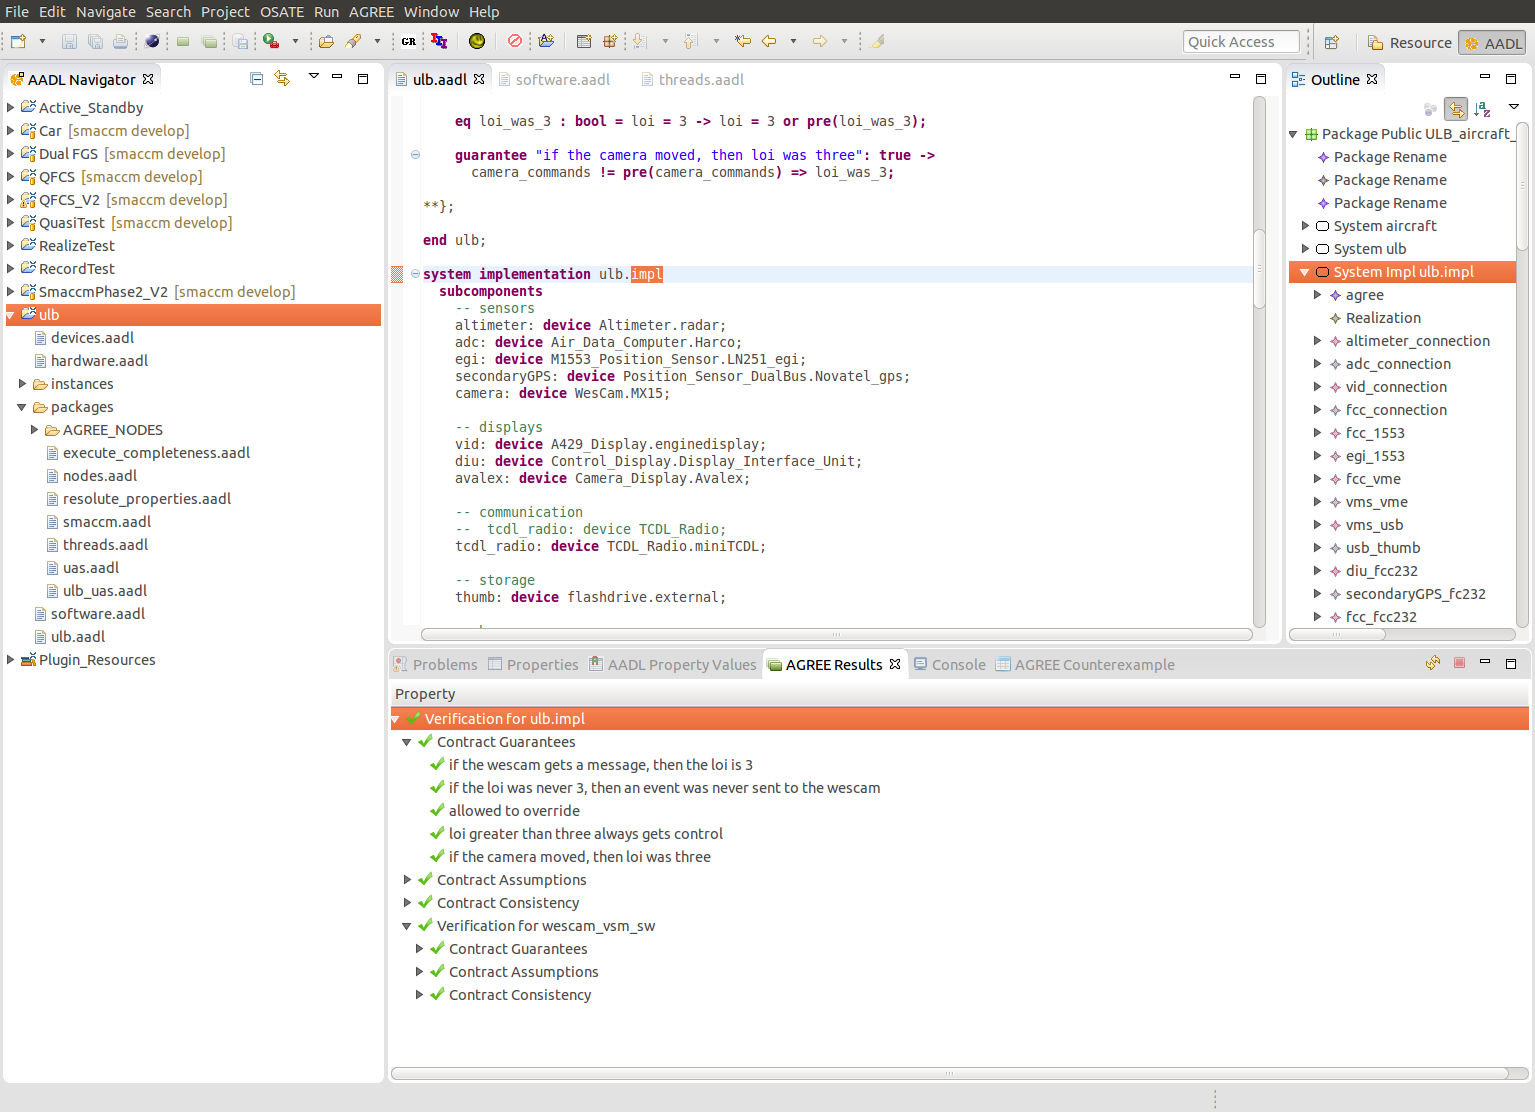
\includegraphics[scale=0.225]{analysis1.png}
\caption{The ULB AADL model in OSATE.  The ULB system implementation is being selected in the outline view on the right hand side of the screen}
\label{fig:osate}
\end{figure}

A results view will appear at the bottom of the screen with the status of all the properties being checked. Results for each component are grouped by guarantees, assumptions, and consistency.  The guarantee and assumption results are the results of checking Formulas~\ref{fml:guar-check} and~\ref{fml:correct-assump}, respectively.  The consistency results check to see if individual contracts can be satisfied over some finite length of time. Checking consistency verifies that the guarantees that you are trying to verify are not vacuously true.  For example, if a subcomponent guarantees ``false'', anything can be proved in the contract of a component containing that subcomponent since it is asserted that the guarantees of a components subcomponents hold.  The consistency check also verifies that the composition of the subcomponents are consistent, and that the contract being analyzed is consistent.

If a counterexample for a property is found then it will have a red icon next to it in the results dialog.  Right-clicking on one of these results will bring up a menu where you can choose to view the counterexample in the console, in a spreadsheet, or in a collapsible menu.  An example of the collapsible menu is shown in Figure~\ref{fig:collapse}.

\begin{figure}
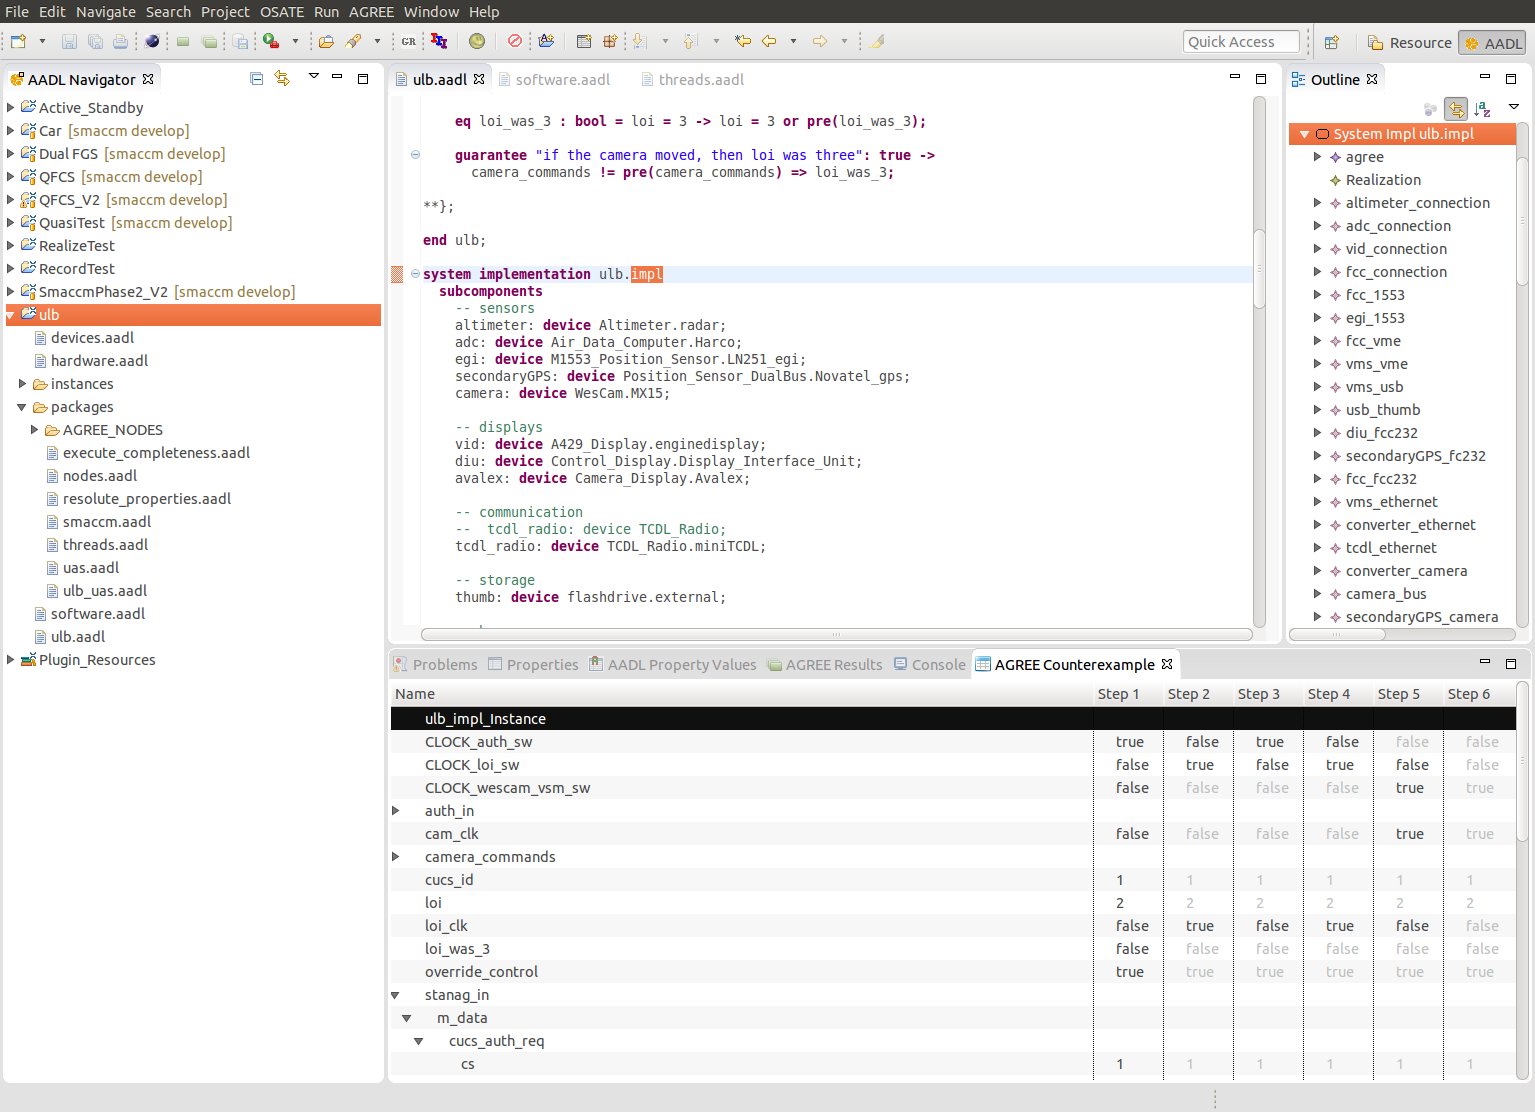
\includegraphics[scale=0.225]{analysis2.png}
\caption{A counterexample being displayed in Eclipse}
\label{fig:collapse}
\end{figure}

There is a preferences menu accessible under Window$\rightarrow$Preferences that can be used to change various options about AGREE's Analysis. This menu is shown in Figure~\ref{fig:prefs}.  Here you can choose between JKind and the Kind2 model checker.  If you choose JKind you can select different SMT Solvers for JKind to use.  You can also decide the timeout and maximum depth for k-induction to use.

\begin{figure}
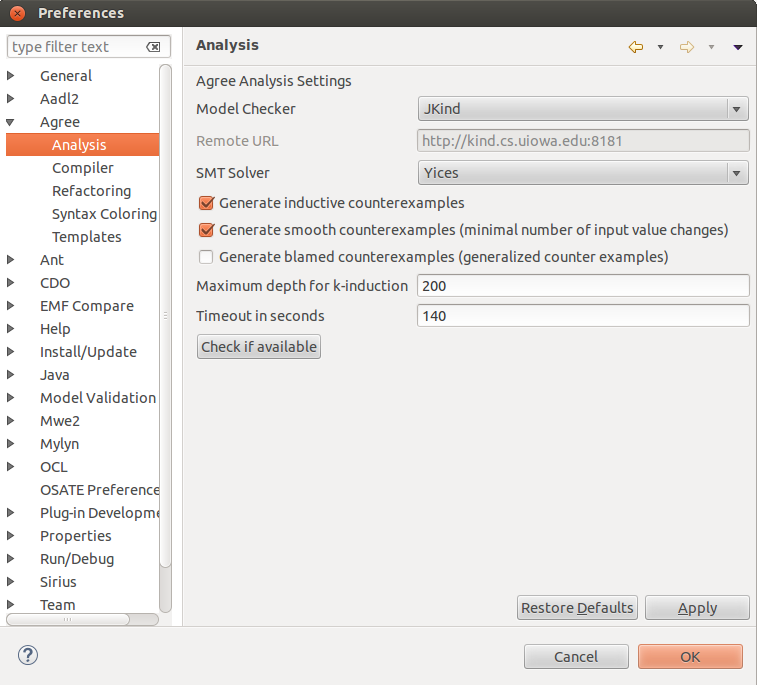
\includegraphics[scale=0.45]{analysis3.png}
\caption{The AGREE preferences menu}
\label{fig:prefs}
\end{figure}

\section{What is left to do?}

Some of the properties that we have proved could be strengthened.  For example, we proved that ``If the camera state changes, then the LOI was three''.  This does not rule out a scenario where the LOI was three, then changed to two, and then the camera changes state from a CUCS authorized with an LOI of two.  A stronger property to prove may be ``Any message sent by a CUCS with LOI not equal to three does not change the camera state''. 

We have neglected to prove more ``liveness-like'' properties at this point because we are unsure of if the quasi-synchronous constraints we have are correct.  For example, we could prove that ``If a CUCS with LOI 3 sends a message to change the state of the camera, the camera state will change in $n$ time steps''.

There are many other aspects of the ULB that could be modelled with AGREE. For example, properties about how the FCC VSM handles STANAG 4586 messages could be verified.  We also need to make sure that the quasi-synchronous constraints that we assumed in our analysis are accurate to the real model.

We did not model any of the messages that the VSM is obligated to return to a CUCS as specified by the STANAG 4586 protocol.  If there are properties of interest with this protocol we could certainly model this.

The analysis that we have done so far assumes that the LOI Manager actually meets the requirements that we have formalized.  The same goes for the requirements that we placed on the Authentication Component, Wescam VSM, and the threads within the Wescam VSM.  In order for the results from AGREE to be accurate, we need to show that the implementations of these components actually meet these requirements.
\end{document}
